\documentclass[a4paper,12pt,oneside,onecolumn]{report}
\usepackage[utf8]{inputenc}
\usepackage{graphicx}
\usepackage[round,numbers]{natbib}
\usepackage{hyperref}
\usepackage{amsmath}
\usepackage{mathtools}
\usepackage{listings}
\usepackage[T1]{fontenc}
\usepackage[scaled=0.9]{beramono}
\usepackage{microtype}
\usepackage{color}
\usepackage{xcolor}
\usepackage{float}
\usepackage{tikz}
\usepackage{pgfplots}
\usepackage{amsfonts}
\usepackage{algorithm}
\usepackage{algorithmic}
\usepackage{listings}

\lstdefinestyle{customAlg}{
	basicstyle=\scriptsize\rmfamily,    
	breakatwhitespace=true,
	breaklines=true,                 
	commentstyle=\color{green!50!black}, 
	escapeinside={\%*}{*)},          
	extendedchars=true,              
	frame=none,                    % adds a frame around the code
	keepspaces=false,                 % keeps spaces in text, useful for keeping indentation of code (possibly needs columns=flexible)
	keywordstyle=\bfseries\color{blue!50!black},       % keyword style
	language=Pascal,                 % the language of the code
	morekeywords={for,output,each,return},
	deletekeywords={new, function, and, set, of, with, record, array},                        
	numbers=left,                    % where to put the line-numbers; possible values are (none, left, right)
	numbersep=3pt,                   % how far the line-numbers are from the code
	numberstyle=\tiny\color{red}, % the style that is used for the line-numbers
	rulecolor=\color{black},         % if not set, the frame-color may be changed on line-breaks within not-black text (e.g. comments (green here))
	showspaces=false,                
	showstringspaces=false,         
	showtabs=false,                  
	tabsize=10,                       % sets default tabsize to 2 spaces
	mathescape=true,
	columns=fullflexible,
	aboveskip=1pt, 
	belowskip=1pt,
}

\lstdefinestyle{customWeka}{
	basicstyle=\scriptsize\rmfamily,    
	breakatwhitespace=true,
	breaklines=true,                 
	commentstyle=\color{green!50!black}, 
	escapeinside={\%*}{*)},          
	extendedchars=true,              
	frame=none,                    % adds a frame around the code
	keepspaces=false,                 % keeps spaces in text, useful for keeping indentation of code (possibly needs columns=flexible)
	keywordstyle=\bfseries\color{blue!50!black},       % keyword style
	morekeywords={Attributes,Instances,Relation,Scheme, Test mode, Number of Leaves, Size of the Tree},
	deletekeywords={new, function, and, set, of, with, record, array},                        
	numbers=none,    % where to put the line-numbers; possible values are (none, left, right)
	rulecolor=\color{black},         % if not set, the frame-color may be changed on line-breaks within not-black text (e.g. comments (green here))
	showspaces=false,                
	showstringspaces=false,         
	showtabs=false,                  
	tabsize=10,                       % sets default tabsize to 2 spaces
	mathescape=true,
	columns=fullflexible,
	aboveskip=1pt, 
	belowskip=1pt,
}

\lstdefinestyle{custWeka2}{
	basicstyle=\scriptsize\rmfamily,    
	breakatwhitespace=true,
	breaklines=true,                 
	commentstyle=\color{green!50!black}, 
	escapeinside={\%*}{*)},          
	extendedchars=true,              
	frame=none,                    % adds a frame around the code
	keepspaces=false,                 % keeps spaces in text, useful for keeping indentation of code (possibly needs columns=flexible)
	keywordstyle=\bfseries\color{blue!50!black},       % keyword style
	morekeywords={FT tree, Number of Leaves, Size of the Tree},
	deletekeywords={new, function, and, set, of, with, record, array},                        
	numbers=none,    % where to put the line-numbers; possible values are (none, left, right)
	rulecolor=\color{black},         % if not set, the frame-color may be changed on line-breaks within not-black text (e.g. comments (green here))
	showspaces=false,                
	showstringspaces=false,         
	showtabs=false,                  
	tabsize=10,                       % sets default tabsize to 2 spaces
	mathescape=true,
	columns=fullflexible,
	aboveskip=1pt, 
	belowskip=1pt,
}


\long\def\symbolfootnote[#1]#2{\begingroup%
\def\thefootnote{\fnsymbol{footnote}}\footnote[#1]{#2}\endgroup}

\usepackage[italian]{babel}
\usepackage{caption}
\captionsetup[table]{name=\textbf{Tabella}}
\captionsetup[figure]{name=\textbf{Figura}}

%\usepackage{tocloft}
%\cftpagenumbersoff{figure}

\title{Documentazione Data Mining} % Title
\author{Simone \textsc{Rutigliano} }
\date{\today}

\usepackage[sans,nowrite,infront,standard,swapnames]{frontespizio}

\begin{document}
	\begin{frontespizio}
		\fontoptionnormal 
		\Universita {Bari}
		\Logo [2cm]{./images/logo}
		\Facolta {Scienze Matematiche, Fisiche e Naturali}
		\Corso [Laurea]{Informatica Magistrale}
		\Titoletto {Data Mining}
		\Titolo {Documentazione progetto}
		\NCandidato{Studente}
		\Candidato{Simone Rutigliano}
		\Annoaccademico {2012-2013}
		\preparefrontpagestandard	%Frontespizio
	\end{frontespizio}

	%\maketitle
	\tableofcontents

	\begingroup
	\renewcommand\numberline[1]{}
	\listoffigures
	\endgroup

	\begingroup
	\renewcommand\numberline[1]{}
	\listoftables
	\endgroup

	\newpage

	\chapter{Introduzione}
Nell'era dell'information Overload, dove giornalmente si producono quantità considerevoli di dati, memorizzati su opportuni database aziendali e non, potrebbe risultare utile utilizzare degli strumenti in grado produrre automaticamente della conoscenza a partire da questa mole di dati. Una metodologia propensa a fare ciò, è la metodologia KDD (\emph{Knowledge Discovery Databases}). 
La prima definizione da attribuire a questa metodologia è stata quella di:

\emph{Intero \textbf{processo} di estrazione di conoscenza, dalla raccolta e pre-processing dei dati, fino alla interpretazione dei risultati"\cite{DBLP:conf/kdd/1995}}


Successivamente Fayyad et al.,hanno raffinato tale definizione trasformandola in: 

\emph{Knowledge discovery is the nontrivial extraction of implicit, previously unknown, and potentially useful information from data.}
\cite{citeulike:1550195} Definendo quindi il processo KDD come un processo in grado di estrarre dai dati delle informazioni non banali, sconosciute e potenzialmente utili. Il processo KDD si articola in diverse fasi cosi come mostrato in figura \ref{kddprocess}.

\begin{figure}[hbtp]
\centering
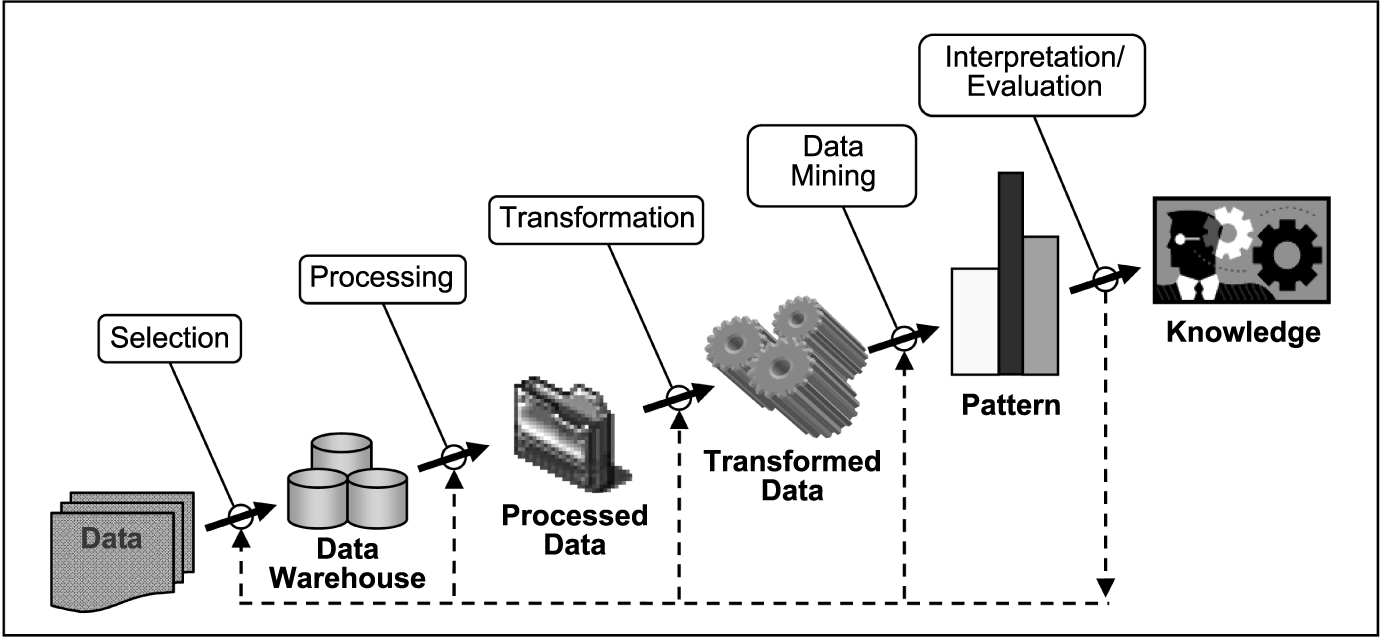
\includegraphics[width=0.9\textwidth]{./images/kddprocess.png}
\caption{Processo KDD}
\label{kddprocess}
\end{figure}

Il Data mining rappresenta la fase principale del processo KDD, il cui compito può consistere o nell'adattare un modello esistente ai dati a disposizione, oppure nel determinare dei possibili pattern ricorrenti tra i dati osservati utilizzando o delle tecniche di machine learning oppure delle tecniche statistiche. 

\section{CRISP-DM}
Per l'applicazione del processo di KDD si seguirà il modello del CRISP-DM (\emph{\textbf{CR}oss \textbf{I}ndustry \textbf{S}tandard \textbf{P}rocess for \textbf{D}ata \textbf{M}ining})
\cite{wirth2000crisp}
, in quanto, tale modello, risulta essere lo standard riconosciuto a livello industriale per la conduzione dei processi di KDD.
Il CRISP-DM si compone di sei fasi il cui ordine non è prestabilito in modo vincolante ma può variare da applicazione ad applicazione. Tipicamente le fasi di cui si compone il modello, vengono eseguite come mostrato in figura \ref{CRISPDM}.

\begin{figure}[hbtp]
\centering
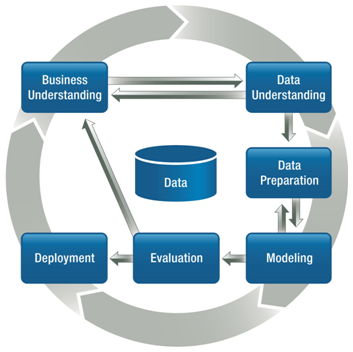
\includegraphics[width=0.6\textwidth]{./images/CRISPDM.png}
\caption{CRISP-DM}
\label{CRISPDM}
\end{figure}

Di seguito verranno esaminate le singole fasi in maniera più approfondita e per ognuna di essa, verrà illustrato l'utilizzo fatto all'interno del contesto del progetto preso in esame.
	\clearpage
	\section{Business Understanding}
Questa fase si focalizza sulla individuazione degli obiettivi e i requisiti del progetto dal punto di vista del business.

\subsection{Background}\label{Background}
Ogni giorno, vengono inviate circa 25 milioni di email indesiderate, chiamate anche email di spam. Tale cifra corrisponde a quasi il 10 \% di tutte le email inviate nel mondo; inoltre, indagini svolte sull'argomento, rivelano che generalmente il 40 \% delle email ricevute giornalmente dai dipendenti di molte imprese risultano essere email di spam, arrivando in alcuni casi, anche al 90 \%.
Queste percentuali risultano essere molto elevate principalmente a causa della facile diffusione delle proprie caselle di posta verso qualunque tipo di contatto, diventando cosi bersagli di messaggi promozionali di qualunque tipo. Questa inondazione di messaggi di spam quindi genera due problemi principali:
\begin{itemize}
\item Saturazione della propria casella di posta, anche se al giorno d'oggi si dispone di una capienza elevata;
\item Perdita di tempo abbastanza considerevole da parte del ricevente nel filtrare queste email.
\end{itemize}


Nel corso degli anni, il desiderio di automatizzare il rilevamento e relativa selezione di queste email di spam, ha portato alla creazione e diffusione di numerosi progetti software e di prodotti commerciali in grado di filtrare lo spam in maniera tutto sommato efficiente; uno dei più diffusi è \textit{SpamAssassin} \footnote{\url{http://spamassassin.apache.org/}}, programma opensource rilasciato sotto licenza Apache 2.0. Si basa su regole di confronto del contesto, supporta anche regole basate su DNS, checksum e filtraggio statistico, inoltre supporta programmi esterni e database online.
SpamAssassin è considerato uno dei filtri antispam più efficaci, specialmente se usato congiuntamente con un database antispam.\cite{wiki:xxx}

\subsubsection{Risorse}
La principale risorsa utilizzata è l'hardware del sistema utilizzato per eseguire l'algoritmo di data mining, in particolar modo, un sistema Windows con un Quad-Core Intel i7 2.00 GHz e 4 GB di Ram.
Il tool di data mining scelto è WEKA (\textbf{W}aikato \textbf{E}nvironment for \textbf{K}nowledge \textbf{A}nalysis) \cite{WEKA}:
una popolare suite di software per il machine learning scritta in Java e sviluppata nell'Università di Waikato (Nuova Zelanda); è stato deciso di utilizzare tale suite, in quanto il software porta con sè i seguenti vantaggi :
\begin{itemize}
	\item Liberamente scaricabile dal sito \footnote{Weka site: \url{http://www.cs.waikato.ac.nz/ml/weka/downloading.html}};
    \item Portabile, in quanto totalmente implementato in java;
    \item Ampia gamma di tecniche di preprocessing e modellazione dei dati;
    \item Facile da usare grazie alla GUI;
\end{itemize}

Per quanto riguarda invece il personale umano, l'unica risorsa umana interpellata nella sperimentazione è lo sperimentatore stesso.

\subsubsection{Vincoli}
	Non sono presenti nè vincoli temporali, nè problemi legali legati alla diffusione del dataset in questione.

\subsubsection{Assunzioni}
	Si assume che i dati di cui si intende disporre siano liberamente accessibili e che non siano falsi o errati.

\subsection{Obiettivi di Business}
	Secondo quanto detto in precedenza, l'obiettivo di business di questo progetto consiste nell'individuazione delle email di spam attraverso l'utilizzo di tecniche di Data Mining.

\subsubsection{Task di Data Mining}
	Il task da realizzare è di tipo \textit{predittivo}, in particolar modo, sarà un task di \textit{classificazione}. L'obiettivo sarà quindi quello di creare un classificatore che sia in grado di etichettare correttamente le nuove email come \textit{spam} o \textit{nospam} sulla base del training set dato in pasto al classificatore. 
\subsection{Criteri di successo}
	Al fine di valutare l'efficacia del classificatore, 
	
	
	Ziel ist es, die Anzahl der durch den Filter hindurch gelassenen Spam-Mails zu minimieren, wobei eine wesentliche Bedingung lautet:
	Unter den ausgefilterten E-Mails dürfen sich maximal 1,0 \% Nicht-Spam-Mails (bezogen auf die Gesamtzahl von Nicht-Spam-Mails) befinden. Achtung: Sollte die eingereichte Lösung diese Bedingung nicht erfüllen, wird die Lösung nicht gewertet!
	
	Folgende Data-Mining-Aufgabe ist zu bearbeiten.
	
	Anhand der Trainingsmenge ist ein Klassifikator zu generieren,
	der auf die exemplarisch ausgewählten 11.177 zu klassifizierenden
	E-Mails anzuwenden ist und oben beschriebenes Problem löst.
	
	Der Klassifikator muss demnach folgende
	Bedingungen erfüllen:
	1. Die Anzahl der Spam-Mails, welche den Filter passieren,
	muss minimiert werden.
	2. Unter den ausgefilterten E-Mails dürfen sich maximal 1,0 \%
	Nicht-Spam-Mails (bezogen auf die Gesamtzahl von Nicht-Spam-Mails)
	befinden.
	
	Achtung: Für die Optimierung des Klassifikators ist zwingend
	die oben angegebene 2. Bedingung (1 \% Klausel) zu
	beachten! Sollte die eingereichte Lösung diese Bedingung
	nicht erfüllen, wird die Lösung nicht gewertet!

\subsection{Glossario dei termini}

\subsection{Analisi Costi-Benefici}

Per quanto riguarda i costi inerenti al processo di KDD, l'unico costo che si avrà, sarà in termini di risorse temporali utilizzate per la realizzazione e relativa verifica dei risultati che il classificatore produrrà.

Invece, i benefici che si otterranno da questo processo, saranno quelli che andranno a sopperire a ciò che è stato detto in precedenza nel paragrafo \ref{Background}.


\subsection{Piano di Progetto}
	\clearpage
	\chapter{Data Understanding}
\begin{figure}[hbtp]
	\centering
	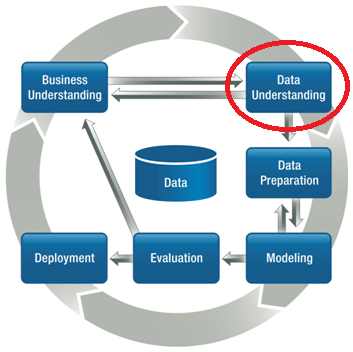
\includegraphics[width=0.5\textwidth]{./images/CRISPDM_2.png}
	\caption{CRISP-DM - Data Understanding}
	\label{CRISPDM_2}
\end{figure}
\section{Raccolta dei dati}
Il dataset preso in esame essendo oggetto della DMC 2003 Competition, è liberamente scaricabile dal sito \url{http://www.data-mining-cup.de/en/review/dmc-2003/}. 

\section{Descrizione dei dati}
Il dataset è composto da 8000 istanze rappresentanti le email. Ogni istanza è caratterizzata da 834 attributi, di cui uno \textit{target}, atto ad etichettare l'istanza come \textit{spam} o \textit{no-spam}, ed un attributo identificativo numerico (\textit{id}). Esempi di attributi utilizzati a rappresentare le istanze delle email sono le seguenti:
%Training set: 8000 Istanze 834 Attributi = 833 + Target
%data\_dmc2003\_train.txt ... 

%Test set: 11177 Istanze da classificare 833 Attributi
%data\_dmc2003\_train.txt.
\begin{table}[hbtp]
	\begin{tabular}{ c | c | c}
		\textbf{Nome attributo} & \textbf{Tipo} & \textbf{Sottotipo} \\
		\hline
		id & Categorico & Nominale \\ 
		ACCEPT\_CREDIT\_CARDS & Categorico & Nominale \\ 
		ACCOUNT\_CLICK & Categorico & Nominale \\ 
		ACT\_NOW & Categorico & Nominale \\ 
		ADDRESSES\_ON\_CD & Categorico & Nominale \\ 
		ADULT\_SITE & Categorico & Nominale \\ 
		ADVERT\_CODE & Categorico & Nominale \\ 
		ADVERT\_CODE2 & Categorico & Nominale \\ 
		ALL\_CAPS\_HEADER & Categorico & Nominale \\ 
		ALL\_CAP\_PORN & Categorico & Nominale \\ 
		ALL\_NATURAL & Categorico & Nominale \\ 
		ALTA\_BUSCADORES\_ES & Categorico & Nominale \\ 
		AMATEUR\_PORN & Categorico & Nominale \\ 
		AMAZING & Categorico & Nominale \\ 
		AMAZING\_STUFF & Categorico & Nominale \\ 
		ANOTHER\_NET\_AD & Categorico & Nominale \\ 
		AOL\_USERS\_LINK & Categorico & Nominale \\ 
		APPLY\_ONLINE & Categorico & Nominale \\ 
		APPROVED\_BY & Categorico & Nominale \\ 
		\vdots  &  \vdots  &  \vdots  \\
	\end{tabular}
\end{table}

Tutti gli attributi, ad esclusione dell'\textit{id} e del \textit{target}, sono di tipo categorico nominale booleano, esso assumerà valore 0 qualora l'email non dovesse averlo, 1 il viceversa.
Il dataset, inoltre, è distribuito in un formato testuale.


\section{Verifica della qualità dei dati}

Il dataset contiene dati di buona qualità in quanto garantiscono le seguenti qualità:

\begin{itemize}
	\item \textbf{Accuratezza}: Il dataset rispecchia perfettamente i dati reali, sono quindi da considerarsi accurati;
	\item \textbf{Completezza}: Considerati i numerosi missing values presenti, molte tuple non sono complete;
	\item \textbf{Consistenza}: I dati sono rappresentati uniformemente nella base di dati. I valori TRUE/FALSE - 0/1 - SI/NO sono stati inseriti utilizzando la sintassi TRUE/FALSE;
	\item \textbf{Attualità dei dati}: I dati sono aggiornati all'anno 2003, anno in cui è stata indetta la KDD Cup nel quale è stato utilizzato questo dataset. Il che potrebbe portare ad una classificazione errata qualora dal 2003 ad oggi, le email di spam fossero cambiate in termini di attributi caratterizzanti queste ultime.
	%Attualità dei dati: I dati non sono aggiornati al 2013 (anno attuale), ma risalgono tutti ad anni passati. Nel caso di IMDB i dati sono aggiornati al 2009, nel caso di UWCSE i dati sono aggiornati al 2004 e nel caso di WEBKB	i dati sono aggiornati al 1997. Ad ogni modo ciò non rappresenta un problema visto che l’obiettivo del KDD process è quello di valutare due versioni di un algoritmo di Data Mining.
\end{itemize}


%Bewertung der Ergebnisse
%------------------------
%
%Der Jury ist bekannt, welche von den 11.177 zu klassifizierenden
%E-Mails tatsächlich Nicht-Spam-Mail oder Spam-Mail ist. Genauer
%gesagt, stammen alle Daten aus einer Stichprobe von insgesamt
%19.177 E-Mails.
%
%Die eingesandten Ergebnisse werden mit der bekannten Information über
%die tatsächliche Zuordnung der E-Mails verglichen und der Anteil der
%nicht ausgefilterten Spam-Mails bestimmt. Gleichzeitig wird der Anteil
%der ausgefilterten Nicht-Spam-Mails ermittelt und die Einhaltung
%der 1 \% Klausel (siehe oben) überprüft. Sieger ist der Teilnehmer
%oder die Teilnehmerin, welche(r) unter Einhaltung der 1 \% Klausel die
%wenigsten Spam-Mails zustellt. Teilnehmer, die die 1 \% Klausel ver-
%letzen, werden nicht gewertet.
%
%La giuria non è noto quali classificare le e-mail è in realtà la posta o spam 11.177 non-spam. In particolare, tutti i dati provengono da un campione totale di 19.177 messaggi di posta elettronica.
%
%I risultati presentati sono confrontati con le informazioni note circa l'assegnazione effettiva delle e-mail e determinata la percentuale di spam non filtrati. Allo stesso tempo, la percentuale di filtrato non spam viene rilevato e il rispetto della clausola 1 \% (vedi sopra) selezionata. Il vincitore è il partecipante o la partecipante, che (r) manda le mail di spam in meno rispetto alla clausola 1 \%. I partecipanti, la clausola 1 \% ferire non saranno conteggiati.
%
%
%I dati contenuti nei tre database sono quasi sempre di alta qualità, ma è bene soffermarsi sulle caratteristiche che questi devono avere:
%
%Completezza: Non sempre tutti i dati sono disponibili. Ci sono alcuni missing values nei tre database.
%IMDB:nella relazione "movies" assume valore nullo l'attributo "budget" (l'informazione non è disponibile).
%UWCSE: nella relazione "persons" spesso assume valore nullo l'attributo "phase" (quando la persona è una matricola o un professore) e nella relazione "prof" talvolta assume valore nullo l'attributo "position" (non è specificata la posizione del professore). 
%Consistenza: I dati sono rappresentati uniformemente nella base di dati. I valori TRUE/FALSE - 0/1 - SI/NO sono stati inseriti utilizzando la sintassi TRUE/FALSE in tutti i database. 
%Attualità dei dati: I dati non sono aggiornati al 2013 (anno attuale), ma risalgono tutti ad anni passati. 
%Nel caso di IMDB i dati sono aggiornati al 2009, nel caso di UWCSE i dati sono aggiornati al 2004 e nel caso di WEBKB i dati sono aggiornati al 1997. Ad ogni modo ciò non rappresenta un problema visto che l’obiettivo del KDD process è quello di valutare due versioni di un algoritmo di Data Mining.Non sono richiesti dati esterni da integrare nelle tre basi di dati.

\section{Esplorazione dei dati}
I dati essendo dei valori booleani indicando la presenza/assenza della feature per quel dato, sono da considerarsi di tipo categorico nominale; Il che porta a poter utilizzare solo grafici in grado di rappresentare la frequenza con cui una feature è presente sui dati. A tale scopo, verranno utilizzati essenzialmente degli istogrammi sugli attributi aventi meno missing value.

\begin{figure}[hbtp]
 	\centering
 	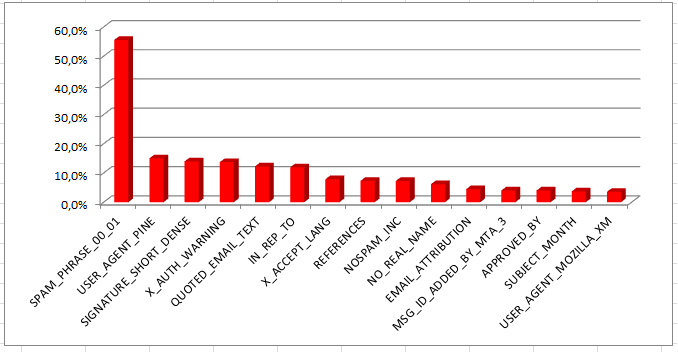
\includegraphics[width=0.9\textwidth]{./images/Histogram_No.png}
 	\caption{Istogramma attributi - Classe No}
 	\label{NoHist}
\end{figure}

\begin{figure}[hbtp]
	\centering
	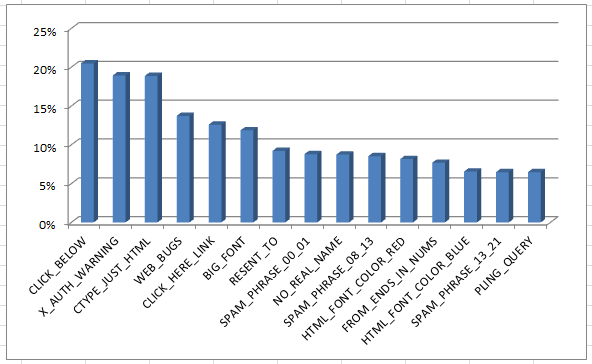
\includegraphics[width=0.9\textwidth]{./images/Histogram_Yes.png}
	\caption{Istogramma attributi - Classe Yes}
	\label{YesHist}
\end{figure}
	\clearpage
    \chapter{Data Preparation}

\begin{figure}[hbtp]
	\centering
	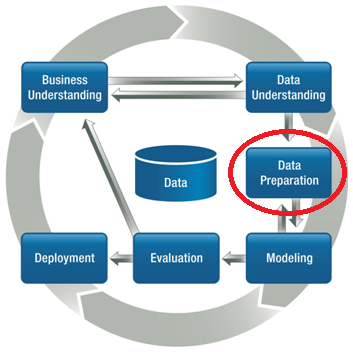
\includegraphics[width=0.5\textwidth]{./images/CRISPDM_3.png}
	\caption{CRISP-DM - Data Preparation}
	\label{CRISPDM_3}
\end{figure}



\section{Criteri di Inclusione/Esclusione dei dati}

\section{Selezione dei dati}

\section{Campionamento}

\section{Feature Selection}

\section{Data Cleaning}

\section{Construct Data}

\section{Integrate Data}

\section{Format Data}

	\clearpage
    \chapter{Modeling}

\begin{figure}[hbtp]
	\centering
	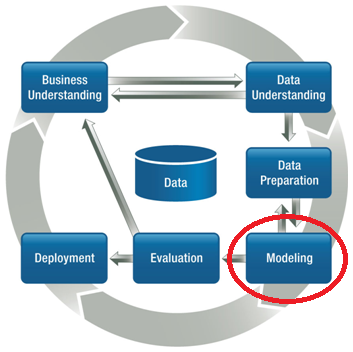
\includegraphics[width=0.5\textwidth]{./images/CRISPDM_4.png}
	\caption{CRISP-DM - Modeling}
	\label{CRISPDM_4}
\end{figure}

\section{Tecnica di Modeling}
Ai fini della classificazione, si è deciso di modellare il dataset realizzando un albero di decisione funzionale. In particolare si è utilizzato l'algoritmo \textbf{FT} (\emph{\textbf{F}unctional \textbf{T}ree}).

\section{Rappresentazione del Modello}
L'algoritmo Functional Tree è un algoritmo di classificazione basato sulla costruzione di alberi 'funzionali', i quali potrebbero avere funzioni di regressione logistica ai nodi e/o alle foglie interne. L'algoritmo, cosi come descritto in \cite{Gama:2004:FT:990375.990395}, è in grado di gestire:
\begin{itemize}
	\item variabili target (binarie o multi-classe)
	\item attributi numerici
	\item attributi nominali
	\item missing values
\end{itemize}
%Classifier for building 'Functional trees', which are classification trees  that could have logistic regression functions at the inner nodes and/or leaves. The algorithm can deal with binary and multi-class target variables, numeric and nominal attributes and missing values.\cite{Gama2004}

\paragraph{Functional Trees}
\subparagraph{Growning phase}
	Dato un set di esempi e un modello di costruzione di nuovi attributi, l'algoritmo generale usato per la creazione dell'albero funzionale risulta essere molto simile all'algoritmo standard per la costruzione degli alberi decisionali, fatta eccezione per alcuni passaggi; In particolare, nella fase di growning, si andranno a creare nuovi attributi derivati dalla valorizzazione delle funzioni di classificazione/regressione costruite sulla base degli attributi originali. Ci sono alcuni aspetti di questo algoritmo che devono essere esplicitati. Innanzitutto il modello verrà costruito usando la funzione costruttore creata tramite l'ausilio degli esempi che ricadono in un determinato nodo. La funzione costruttore deve essere un classificatore o un regressore, a seconda della tipologia di task da risolvere. Ogni nuovo attributo è computato come valore predetto dalla funzione costruita per ogni esempio. In caso di classificazione, ogni nuovo valore di questo attributo sarà ottenuto calcolando la probabilità che quell'esempio appartenga a una delle classi date (\emph{LinearBayes Classifier} \cite{DBLP:conf/sbia/Gama00}; Per fare ciò, si andrà a utilizzare la funzione di merito di un albero univariato tenendo conto sempre dei valori originali degli attributi (i.e. \emph{Gain Ratio}). Una volta creati, questi nuovi attributi verranno utilizzati per la creazione del modello finale. Inoltre, la cardinalità dei nuovi attributi da creare sarà pari al quantitativo di classi che si hanno a disposizione.
	Il modello costruito dall'algoritmo potrà avere due tipologie di nodi decisionali: 
	\begin{itemize}
		\item nodi basati sul test eseguiti su un attributo originale;
		\item nodi valorizzati sulla base della funzione costruita.
	\end{itemize} 
	Nel secondo caso, si andrà a usare un modello lineare generalizzato per costruire i nuovi attributi; in questo caso, ogni nuovo attributo è ottenuto tramite combinazione lineare degli attributi di partenza. I nodi decisionali basati sui nuovi attributi, pertanto, permettono di definire un piano di decisione multivariato.

%\begin{figure}[hbtp]
%	\centering
%	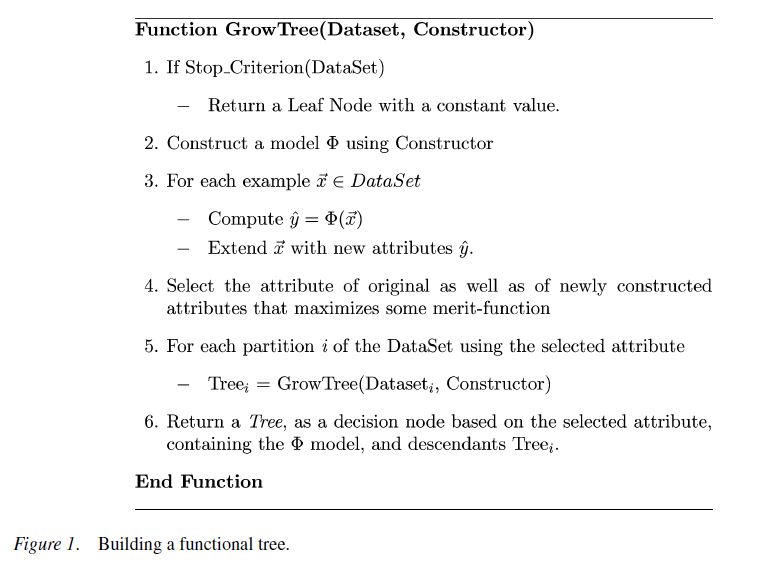
\includegraphics[width=0.9\textwidth]{./images/FunctionGrowTree.JPG}
%	\caption{Function GrowTree}
%\end{figure}

\lstset{style=customAlg}
\begin{algorithm}
	\caption{Function GrowTree(Dataset, Constructor)}
	\begin{lstlisting}
  If $Stop\_Criterion(DataSet)$
     Return a Leaf Node with a constant value.
  Construct a model $\Phi$ using Constructor
  For each example $\vec{x} \in DataSet$
     Compute $\hat y = \Phi(\vec{x})$
     Extend $\vec{x}$ with new attributes $\hat y$.
  Select the attribute of original as well as of newly constructed attributes that maximizes some merit-function
  For each partition $i$ of the DataSet using the selected attribute
     $Tree_{i} = GrowTree (Dataset_{i},Constructor)$
  Return a $Tree$, as a decision node based on the selected attribute, contaning the $\Phi$ model, and descendants $Tree_{i}$.
	\end{lstlisting}
\end{algorithm}

\subparagraph{Prune Phase}
	Una volta creato l'albero, si passerà alla fase di pruning in modo tale da ridurre l'overfitting dell'albero sul training set. L'algoritmo prevede la visita dell'albero usando un approccio bottom-up (Post-visita). Per ogni nodo non foglia vengono stimati due valori quantitativi: 
\begin{itemize}
	\item errore statico
	\item errore di Backed-up
\end{itemize}
L'\emph{errore statico} indica la probabilità di misclassification ad un nodo $v$ ignorando i suoi sottoalberi figli.
$$e(v) = P (class \neq C)|v$$
L'\emph{errore di backed-up}, invece, è la somma pesata della stima degli errori di tutti i sotto alberi del nodo corrente $v$. La stima dell'errore di ogni ramo è pesato usando la probabilità che un esempio appartenga al ramo.
$$E(T)=p_1E(T_1)+p_2E(T_2)+\dots$$ 
Se l'errore di backed-up dovesse essere maggiore o uguale dell'errore statico, il nodo verrà sostituito da una foglia avente come valore, il valore attribuito dalla classe di maggioranza del nodo.
L'errore a $T$ diventerà quindi il minimo trai 2 errori calcolati in precedenza.
$$ E(T) = \min \left( e \left( v \right), ~ \sum_i p_i E \left( T_i \right) \right) $$
L'aspetto fondamentale dell'algoritmo di potatura è l'errore stimato nella fase 1. Ad ogni nodo, sarà necessario stimare la probabilità dell'errore dato l'errore nel campione degli esempi che ricadono in questo nodo; inoltre, tale probabilità non può essere determinata con certezza. A tale scopo, per un dato livello di precisione, consideriamo un intervallo di confidenza $\left[L_{cf}~;~U_{cf}\right]$ con una probabilità di $1-cf$ che contenga l'errore reale. Cosi come in \cite{Quinlan:1993a}, il limite superiore dell'intervallo di confidenza ($U_{cf}$), ottenuto tramite errore di campionamento della distribuzione, sta a indicare la \emph{stima pessimistica} dell'errore reale. L'intervallo di confidenza per l'errore dipende dalla funzione di perdita\footnote{ La funzione di perdita riflette le conseguenze negative associate alla decisione "sbagliata"} usata. In caso di classificazione, con perdita 0-1, l'errore seguirà una distribuzione binomiale \cite{mitchellbook}.
Una procedura simile è utilizzata per stimare l'errore di costruzione ($Constructor\_Error$).

% \begin{figure}[hbtp]
% 	\centering
% 	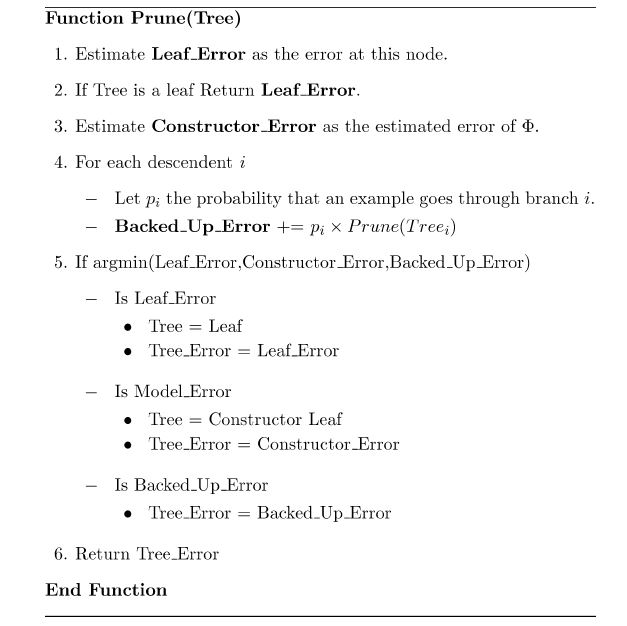
\includegraphics[width=0.5\textwidth]{./images/FunctionGrowTreePrune.JPG}
% 	\caption{Function GrowTree Prune}
% \end{figure}

\begin{algorithm}
	\caption{Function Prune (Tree)}
	\begin{lstlisting}
  Estimate Leaf_Error as the error at this node
  If Tree is leaf 
     Return Leaf_Error
  Estimate Constructor_Error as the estimated error of $\Phi$
  For each descendent $i$
     Let $p_i$ the probability that an example goes through branch $i$
     Backed_Up_Error $+= p_i \times Prune \left(Tree_i\right)$
  If argmin (Leaf_Error, Constructor_Error, Backed_up_error)
     Is Leaf_Error
        Tree = Leaf
        Tree_Error = Leaf_Error
     Is Model Error
        Tree = Constructor Leaf
        Tree_Error = Constructor_Error
     Is Backed_Up_Error
        Tree_Error = Backed_Up_Error
	\end{lstlisting}
\end{algorithm}
L'algoritmo di potatura sarà in grado di produrre due diversi tipi di foglie: 
\begin{itemize}
	\item Nodi foglia in grado di predire direttamente la classe da attribuire al nuovo esempio, nel caso in cui $$\min (E_{Backed\_Up}~,~E_{Static\_Error}) < E_{Constructor\_Error}$$	
	\item Nodi foglia contenenti la funzione costruttrice creata in fase di growing in quel nodo, nel caso in cui
	$$\min (E_{Backed\_Up}~,~E_{Static\_Error}) > E_{Constructor\_Error}$$
\end{itemize}
Si ottengono cosi due modelli concettualmente differenti in base a questa differenziazione, più un terzo modello ibrido.

\paragraph{Alberi funzionali ai soli nodi foglia}
\label{Alberi funzionali ai soli nodi foglia}
Utilizzando l'approccio FT-Leaves, il modello funzionale non viene utilizzato nei test per effettuare lo splitting, ma solo ed esclusivamente nelle foglie. In questo approccio, si restringe la selezione degli attributi di test ai soli attributi di partenza.
Questo è l'approccio utilizzato ad esempio nell'M5 di Quinlan \cite{DBLP:conf/icml/Quinlan93}, e nel sistema NBtree \cite{Kohavi1996}. 
Tuttavia, a ogni nodo viene costruita la funzione costruttore che verrà poi utilizzata nella fase di pruning dell'albero. In questo modo, tutti i nodi decisionali sono basati sugli attributi di partenza, ma anche i nodi foglia potrebbero contenere il modello costruttore se e solo se, nell'algoritmo di pruning, l'errore stimato del modello costruttore risulti essere inferiore sia all'errore di backed-up che all'errore statico. Un albero funzionale FT-Leaves divide lo spazio di input in iper-rettagoli. I dati in ogni regione vengono adattati usando la funzione costruttore.

\paragraph{Alberi funzionali ai soli nodi intermedi}
\label{Alberi funzionali ai soli nodi intermedi}
Utilizzando l'approccio FT-Inner, si otterranno degli alberi funzionali nel quale i modelli multivariati verranno usati esclusivamente ai nodi decisionali (nodi interni) e non verranno mai usati come classificatori nei nodi foglia. In questo caso, l'algoritmo di pruning verrà limitato alla sola scelta tra l'errore di  Backed-up e l'errore statico, facendo in modo che, nelle foglie, siano presenti solo i valori costanti utili alla classificazione diretta. Questo approccio è utilizzato in sistemi come LTREE \cite{Gama97}. Un albero funzionale FT-Inner divide lo spazio di input in superfici decisionali oblique. I dati in ogni regione vengono adattati usando la costante che minimizzi la funzione di perdita data.
%\paragraph{Functional inner nodes only} We denote as FT-Inner the approach to functional trees where the multivariate models are used exclusively at decision nodes (internal nodes) and not used as classifiers in leaves. In our algorithm, restricting the pruning algorithm to choose only between the Backed-up-Error and the Static error generates this kind of model. In this case all leaves predict a constant value. This is the strategy used in systems like LMDT (Utgoff & Brodley, 1991), OC1 (Murthy, Kasif, & Salzberg, 1994), LTREE (Gama, 1997), and QUEST (Loh & Shih, 1997). A FT-Inner functional tree divides the input space into oblique decision surfaces. The data in each region is fitted with a constant that minimizes the given loss function. %
\paragraph{Alberi funzionali ibridi}
\label{FT Hybrid}
Combinando i due approcci descritti nei paragrafi precedenti, si ottiene un approccio ibrido nel quale è possibile avere il modello costruttore sia alle foglie che ai nodi intermedi senza nessun vincolo nè in fase di costruzione, nè in fase di potatura. Questo approccio prende il nome di \emph{FT model}.

\paragraph{Predire usando gli alberi funzionali}
Una volta ultimato l'algoritmo di creazione dell'albero (crescita e successiva potatura), questo viene usato per predire il valore di un attributo target su un esempio non classificato. Per fare ciò, l'esempio attraversa l'albero funzionale in modalità top-down (dal nodo radice al nodo foglia). Ad ogni nodo decisionale (inner node) dell'albero, il set di attributi dell'esempio viene esteso usando la funzione costruttore creata a quel nodo. Dopo questa espansione, il test decisionale del nodo viene applicato definendo il percorso che l'esempio dovrà seguire. Una volta che si raggiungerà un nodo foglia, l'esempio verrà classificato o secondo la costante associata al nodo foglia, oppure alla funzione costruttrice creata in quel nodo.

\section{Costruzione del Modello}
I parametri impostati per l'algoritmo Functional Tree in weka, saranno i seguenti:
\begin{multicols}{2}
\begin{itemize}
	\item binSplit: False
	\item debug: False
	\item errorOnProbabilities: False
	\item minNumInstances: 15
	\item \textbf{modelType}: \textbf{FT}
	\item numBoostingIterations: 15
	\item useAIC: False
	\item weightTrimBeta: 0.0
\end{itemize}
\end{multicols}

Il modello seguente è stato costruito usando la configurazione:
\begin{itemize}
	\item feature selection fatta con CfsSubsetEval (\ref{Feature Selection})
	\item sampling fatto con SMOTE (\ref{SMOTE})
	\item approccio ibrido FT (\ref{FT Hybrid})
\end{itemize}	
{\footnotesize
\begin{verbatim}
=== Run information ===

Scheme:     weka.classifiers.trees.FT -I 15 -F 0 -M 15 -W 0.0

Relation:   SPAM-weka.filters.supervised.instance.SMOTE-C0-K5-P100.0-S1-
            weka.filters.supervised.attribute.AttributeSelection-
            Eweka.attributeSelection.CfsSubsetEval-
            Sweka.attributeSelection.BestFirst -D 1 -N 5

Instances:  11112

Attributes: 53	
\end{verbatim}
\begin{multicols}{2}
	\begin{verbatim}
	id
	APPROVED_BY
	BASE64_ENC_TEXT
	BIG_FONT
	CLICK_BELOW
	CRON_ENV
	CTYPE_JUST_HTML
	DATE_IN_FUTURE_06_12
	DATE_IN_PAST_06_12
	DIET
	DOMAIN_4U2
	EXCHANGE_SERVER
	EXCUSE_14
	EXCUSE_3
	FAILURE_NOTICE_2
	FORGED_HOTMAIL_RCVD
	FORGED_YAHOO_RCVD
	FROM_ENDS_IN_NUMS
	HTML_FONT_COLOR_GRAY
	HTML_FONT_INVISIBLE
	HTML_WITH_BGCOLOR
	INVALID_DATE
	KNOWN_MAILING_LIST
	LINES_OF_YELLING
	MAILTO_TO_REMOVE
	MAY_BE_FORGED
	MIME_HTML_NO_CHARSET
	MISSING_MIMEOLE
	MORTGAGE_OBFU
	MSG_ID_ADDED_BY_MTA_2
	NORMAL_HTTP_TO_IP
	NO_REAL_NAME
	ONLY_COST
	PLING_QUERY
	QUOTED_EMAIL_TEXT
	REMOVE_PAGE
	RESENT_TO
	RISK_FREE
	SAVE_MONEY
	SIGNATURE_LONG_DENSE
	SIGNATURE_SHORT_SPARSE
	SPAM_PHRASE_00_01
	SPAM_PHRASE_08_13
	SUBJECT_MONTH
	SUBJ_ALL_CAPS
	TRACKER_ID
	UNSUB_PAGE
	USER_AGENT_PINE
	USER_AGENT_TONLINE
	USER_IN_WHITELIST
	WEB_BUGS
	X_ACCEPT_LANG
	target
	Test mode:10-fold cross-validation
	\end{verbatim}
\end{multicols}
\begin{verbatim}
	=== Classifier model (full training set) ===
	
	FT tree 
	------------------
	
	N0#1 <= 0.618916
	|   id <= 372407
	|   |   N0#3 <= 0.156641: FT_1:15/60 (4856)
	|   |   N0#3 > 0.156641
	|   |   |   N0#5 <= 0.825819
	|   |   |   |   N0#6 <= 0.513027: Class=1
	|   |   |   |   N0#6 > 0.513027: FT_3:15/90 (32)
	|   |   |   N0#5 > 0.825819: FT_4:15/75 (121)
	|   id > 372407: Class=0
	N0#1 > 0.618916
	|   N0#11 <= 0.865508: FT_6:15/45 (34)
	|   N0#11 > 0.865508
	|   |   N0#13 <= 0.995526
	|   |   |   N0#14 <= 0.973489: FT_7:15/75 (68)
	|   |   |   N0#14 > 0.973489: FT_8:15/75 (267)
	|   |   N0#13 > 0.995526: Class=0
	
	Number of Leaves  : 	9
	
	Size of the Tree : 	17
\end{verbatim}
\pagebreak
\begin{multicols}{2}
	\begin{verbatim}
		FT_N0#1:
		Class 0 :
		-1.07 + 
		[id] * 0    +
		[BASE64_ENC_TEXT] * 2.03 +
		[BIG_FONT] * 0.88 +
		[CLICK_BELOW] * 0.9  +
		[CTYPE_JUST_HTML] * 2.17 +
		[FROM_ENDS_IN_NUMS] * 0.77 +
		[INVALID_DATE] * 1.11 +
		[MISSING_MIMEOLE] * 1.1  +
		[RESENT_TO] * 1.14 +
		[SPAM_PHRASE_00_01] * -1.44 +
		[USER_AGENT_PINE] * -0.72 +
		[WEB_BUGS] * 0.97 +
		[X_ACCEPT_LANG] * -0.72
		
		Class 1 :
		1.07 + 
		[id] * 0    +
		[BASE64_ENC_TEXT] * -2.03 +
		[BIG_FONT] * -0.88 +
		[CLICK_BELOW] * -0.9 +
		[CTYPE_JUST_HTML] * -2.17 +
		[FROM_ENDS_IN_NUMS] * -0.77 +
		[INVALID_DATE] * -1.11 +
		[MISSING_MIMEOLE] * -1.1 +
		[RESENT_TO] * -1.14 +
		[SPAM_PHRASE_00_01] * 1.44 +
		[USER_AGENT_PINE] * 0.72 +
		[WEB_BUGS] * -0.97 +
		[X_ACCEPT_LANG] * 0.72
		
		
		FT_N0#3:
		Class 0 :
		-1.52 + 
		[id] * 0    +
		[APPROVED_BY] * -0.53 +
		[BASE64_ENC_TEXT] * 3.04 +
		[BIG_FONT] * 0.88 +
		[CLICK_BELOW] * 0.9  +
		[CTYPE_JUST_HTML] * 4.01 +
		[DATE_IN_FUTURE_06_12] * 1.09 +
		[DIET] * 1.37 +
		[EXCHANGE_SERVER] * -0.52 +
		[EXCUSE_3] * 0.92 +
		[FORGED_HOTMAIL_RCVD] * 1.32 +
		[FORGED_YAHOO_RCVD] * 1.39 +
		[FROM_ENDS_IN_NUMS] * 0.77 +
		[HTML_FONT_COLOR_GRAY] * -0.97 +
		[INVALID_DATE] * 1.11 +
		[KNOWN_MAILING_LIST] * -0.68 +
		[MIME_HTML_NO_CHARSET] * 1.11 +
		[MISSING_MIMEOLE] * 2.16 +
		[MSG_ID_ADDED_BY_MTA_2] * 0.87 +
		[NORMAL_HTTP_TO_IP] * 1.53 +
		[ONLY_COST] * 1.44 +
		[PLING_QUERY] * 1.32 +
		[QUOTED_EMAIL_TEXT] * -1.06 +
		[REMOVE_PAGE] * 1.43 +
		[RESENT_TO] * 2.03 +
		[RISK_FREE] * 1.65 +
		[SPAM_PHRASE_00_01] * -0.76 +
		[SPAM_PHRASE_08_13] * 1.31 +
		[SUBJECT_MONTH] * -0.46 +
		[TRACKER_ID] * 1.3  +
		[USER_AGENT_PINE] * -1.26 +
		[WEB_BUGS] * 0.97 +
		[X_ACCEPT_LANG] * -1.37
		
		Class 1 :
		1.52 + 
		[id] * 0    +
		[APPROVED_BY] * 0.53 +
		[BASE64_ENC_TEXT] * -3.04 +
		[BIG_FONT] * -0.88 +
		[CLICK_BELOW] * -0.9 +
		[CTYPE_JUST_HTML] * -4.01 +
		[DATE_IN_FUTURE_06_12] * -1.09 +
		[DIET] * -1.37 +
		[EXCHANGE_SERVER] * 0.52 +
		[EXCUSE_3] * -0.92 +
		[FORGED_HOTMAIL_RCVD] * -1.32 +
		[FORGED_YAHOO_RCVD] * -1.39 +
		[FROM_ENDS_IN_NUMS] * -0.77 +
		[HTML_FONT_COLOR_GRAY] * 0.97 +
		[INVALID_DATE] * -1.11 +
		[KNOWN_MAILING_LIST] * 0.68 +
		[MIME_HTML_NO_CHARSET] * -1.11 +
		[MISSING_MIMEOLE] * -2.16 +
		[MSG_ID_ADDED_BY_MTA_2] * -0.87 +
		[NORMAL_HTTP_TO_IP] * -1.53 +
		[ONLY_COST] * -1.44 +
		[PLING_QUERY] * -1.32 +
		[QUOTED_EMAIL_TEXT] * 1.06 +
		[REMOVE_PAGE] * -1.43 +
		[RESENT_TO] * -2.03 +
		[RISK_FREE] * -1.65 +
		[SPAM_PHRASE_00_01] * 0.76 +
		[SPAM_PHRASE_08_13] * -1.31 +
		[SUBJECT_MONTH] * 0.46 +
		[TRACKER_ID] * -1.3 +
		[USER_AGENT_PINE] * 1.26 +
		[WEB_BUGS] * -0.97 +
		[X_ACCEPT_LANG] * 1.37
		
		FT_1:
		Class 0 :
		-1.95 + 
		[id] * 0    +
		[APPROVED_BY] * -1.04 +
		[BASE64_ENC_TEXT] * 3.04 +
		[BIG_FONT] * 0.88 +
		[CLICK_BELOW] * 4.97 +
		[CRON_ENV] * -0.54 +
		[CTYPE_JUST_HTML] * 31.85 +
		[DATE_IN_FUTURE_06_12] * 1.09 +
		[DIET] * 1.37 +
		[EXCHANGE_SERVER] * -0.52 +
		[EXCUSE_3] * 0.92 +
		[FORGED_HOTMAIL_RCVD] * 1.32 +
		[FORGED_YAHOO_RCVD] * 2.9  +
		[FROM_ENDS_IN_NUMS] * 0.36 +
		[HTML_FONT_COLOR_GRAY] * -0.97 +
		[INVALID_DATE] * 1.11 +
		[KNOWN_MAILING_LIST] * -0.68 +
		[MIME_HTML_NO_CHARSET] * 1.11 +
		[MISSING_MIMEOLE] * 2.16 +
		[MORTGAGE_OBFU] * 2.78 +
		[MSG_ID_ADDED_BY_MTA_2] * 0.87 +
		[NORMAL_HTTP_TO_IP] * 1.53 +
		[ONLY_COST] * 1.44 +
		[PLING_QUERY] * 1.32 +
		[QUOTED_EMAIL_TEXT] * -1.58 +
		[REMOVE_PAGE] * 1.43 +
		[RESENT_TO] * 2.03 +
		[RISK_FREE] * 1.65 +
		[SPAM_PHRASE_00_01] * -0.48 +
		[SPAM_PHRASE_08_13] * 1.31 +
		[SUBJECT_MONTH] * -1.83 +
		[TRACKER_ID] * 5.74 +
		[USER_AGENT_PINE] * -2.01 +
		[WEB_BUGS] * 0.97 +
		[X_ACCEPT_LANG] * -1.37
		
		Class 1 :
		1.95 + 
		[id] * 0    +
		[APPROVED_BY] * 1.04 +
		[BASE64_ENC_TEXT] * -3.04 +
		[BIG_FONT] * -0.88 +
		[CLICK_BELOW] * -4.97 +
		[CRON_ENV] * 0.54 +
		[CTYPE_JUST_HTML] * -31.85 +
		[DATE_IN_FUTURE_06_12] * -1.09 +
		[DIET] * -1.37 +
		[EXCHANGE_SERVER] * 0.52 +
		[EXCUSE_3] * -0.92 +
		[FORGED_HOTMAIL_RCVD] * -1.32 +
		[FORGED_YAHOO_RCVD] * -2.9 +
		[FROM_ENDS_IN_NUMS] * -0.36 +
		[HTML_FONT_COLOR_GRAY] * 0.97 +
		[INVALID_DATE] * -1.11 +
		[KNOWN_MAILING_LIST] * 0.68 +
		[MIME_HTML_NO_CHARSET] * -1.11 +
		[MISSING_MIMEOLE] * -2.16 +
		[MORTGAGE_OBFU] * -2.78 +
		[MSG_ID_ADDED_BY_MTA_2] * -0.87 +
		[NORMAL_HTTP_TO_IP] * -1.53 +
		[ONLY_COST] * -1.44 +
		[PLING_QUERY] * -1.32 +
		[QUOTED_EMAIL_TEXT] * 1.58 +
		[REMOVE_PAGE] * -1.43 +
		[RESENT_TO] * -2.03 +
		[RISK_FREE] * -1.65 +
		[SPAM_PHRASE_00_01] * 0.48 +
		[SPAM_PHRASE_08_13] * -1.31 +
		[SUBJECT_MONTH] * 1.83 +
		[TRACKER_ID] * -5.74 +
		[USER_AGENT_PINE] * 2.01 +
		[WEB_BUGS] * -0.97 +
		[X_ACCEPT_LANG] * 1.37
		
		FT_N0#5:
		Class 0 :
		-0.59 + 
		[APPROVED_BY] * -0.53 +
		[BASE64_ENC_TEXT] * 3.04 +
		[BIG_FONT] * 0.88 +
		[CLICK_BELOW] * 0.9  +
		[CTYPE_JUST_HTML] * 4.01 +
		[DATE_IN_FUTURE_06_12] * 1.09 +
		[DIET] * 2.22 +
		[EXCHANGE_SERVER] * -1.6 +
		[EXCUSE_3] * 0.92 +
		[FORGED_HOTMAIL_RCVD] * 1.32 +
		[FORGED_YAHOO_RCVD] * 0.96 +
		[FROM_ENDS_IN_NUMS] * 0.77 +
		[HTML_FONT_COLOR_GRAY] * -1.85 +
		[HTML_FONT_INVISIBLE] * -1 +
		[INVALID_DATE] * 1.11 +
		[KNOWN_MAILING_LIST] * -2.32 +
		[MIME_HTML_NO_CHARSET] * 1.11 +
		[MISSING_MIMEOLE] * 2.16 +
		[MSG_ID_ADDED_BY_MTA_2] * 0.39 +
		[NORMAL_HTTP_TO_IP] * 1.53 +
		[ONLY_COST] * 2.25 +
		[PLING_QUERY] * 2.37 +
		[QUOTED_EMAIL_TEXT] * -1.06 +
		[REMOVE_PAGE] * 1.43 +
		[RESENT_TO] * 2.03 +
		[RISK_FREE] * 2.57 +
		[SPAM_PHRASE_00_01] * -0.33 +
		[SPAM_PHRASE_08_13] * 1.31 +
		[SUBJECT_MONTH] * -0.46 +
		[TRACKER_ID] * 1.3  +
		[USER_AGENT_PINE] * -3.23 +
		[WEB_BUGS] * 0.97 +
		[X_ACCEPT_LANG] * -1.37
		
		Class 1 :
		0.59 + 
		[APPROVED_BY] * 0.53 +
		[BASE64_ENC_TEXT] * -3.04 +
		[BIG_FONT] * -0.88 +
		[CLICK_BELOW] * -0.9 +
		[CTYPE_JUST_HTML] * -4.01 +
		[DATE_IN_FUTURE_06_12] * -1.09 +
		[DIET] * -2.22 +
		[EXCHANGE_SERVER] * 1.6  +
		[EXCUSE_3] * -0.92 +
		[FORGED_HOTMAIL_RCVD] * -1.32 +
		[FORGED_YAHOO_RCVD] * -0.96 +
		[FROM_ENDS_IN_NUMS] * -0.77 +
		[HTML_FONT_COLOR_GRAY] * 1.85 +
		[HTML_FONT_INVISIBLE] * 1    +
		[INVALID_DATE] * -1.11 +
		[KNOWN_MAILING_LIST] * 2.32 +
		[MIME_HTML_NO_CHARSET] * -1.11 +
		[MISSING_MIMEOLE] * -2.16 +
		[MSG_ID_ADDED_BY_MTA_2] * -0.39 +
		[NORMAL_HTTP_TO_IP] * -1.53 +
		[ONLY_COST] * -2.25 +
		[PLING_QUERY] * -2.37 +
		[QUOTED_EMAIL_TEXT] * 1.06 +
		[REMOVE_PAGE] * -1.43 +
		[RESENT_TO] * -2.03 +
		[RISK_FREE] * -2.57 +
		[SPAM_PHRASE_00_01] * 0.33 +
		[SPAM_PHRASE_08_13] * -1.31 +
		[SUBJECT_MONTH] * 0.46 +
		[TRACKER_ID] * -1.3 +
		[USER_AGENT_PINE] * 3.23 +
		[WEB_BUGS] * -0.97 +
		[X_ACCEPT_LANG] * 1.37
		
		FT_N0#6:
		Class 0 :
		-0.78 + 
		[APPROVED_BY] * -0.53 +
		[BASE64_ENC_TEXT] * 3.04 +
		[BIG_FONT] * 0.88 +
		[CLICK_BELOW] * 11.29 +
		[CTYPE_JUST_HTML] * 4.01 +
		[DATE_IN_FUTURE_06_12] * 0.23 +
		[DATE_IN_PAST_06_12] * 0.7  +
		[DIET] * 2.22 +
		[EXCHANGE_SERVER] * -1.6 +
		[EXCUSE_14] * 2.03 +
		[EXCUSE_3] * 1.57 +
		[FORGED_HOTMAIL_RCVD] * 1.32 +
		[FORGED_YAHOO_RCVD] * 0.96 +
		[FROM_ENDS_IN_NUMS] * 0.77 +
		[HTML_FONT_COLOR_GRAY] * -2.78 +
		[HTML_FONT_INVISIBLE] * -1 +
		[INVALID_DATE] * 1.11 +
		[KNOWN_MAILING_LIST] * -2.32 +
		[LINES_OF_YELLING] * -1.36 +
		[MIME_HTML_NO_CHARSET] * 1.11 +
		[MISSING_MIMEOLE] * 2.16 +
		[MSG_ID_ADDED_BY_MTA_2] * 0.39 +
		[NORMAL_HTTP_TO_IP] * 1.53 +
		[ONLY_COST] * 2.25 +
		[PLING_QUERY] * 2.37 +
		[QUOTED_EMAIL_TEXT] * -1.06 +
		[REMOVE_PAGE] * 1.43 +
		[RESENT_TO] * 1.43 +
		[RISK_FREE] * 2.57 +
		[SPAM_PHRASE_00_01] * -0.33 +
		[SPAM_PHRASE_08_13] * 0.76 +
		[SUBJECT_MONTH] * 0.89 +
		[SUBJ_ALL_CAPS] * 1.53 +
		[TRACKER_ID] * 2.21 +
		[USER_AGENT_PINE] * -3.23 +
		[WEB_BUGS] * 0.97 +
		[X_ACCEPT_LANG] * -1.37
		
		Class 1 :
		0.78 + 
		[APPROVED_BY] * 0.53 +
		[BASE64_ENC_TEXT] * -3.04 +
		[BIG_FONT] * -0.88 +
		[CLICK_BELOW] * -11.29 +
		[CTYPE_JUST_HTML] * -4.01 +
		[DATE_IN_FUTURE_06_12] * -0.23 +
		[DATE_IN_PAST_06_12] * -0.7 +
		[DIET] * -2.22 +
		[EXCHANGE_SERVER] * 1.6  +
		[EXCUSE_14] * -2.03 +
		[EXCUSE_3] * -1.57 +
		[FORGED_HOTMAIL_RCVD] * -1.32 +
		[FORGED_YAHOO_RCVD] * -0.96 +
		[FROM_ENDS_IN_NUMS] * -0.77 +
		[HTML_FONT_COLOR_GRAY] * 2.78 +
		[HTML_FONT_INVISIBLE] * 1    +
		[INVALID_DATE] * -1.11 +
		[KNOWN_MAILING_LIST] * 2.32 +
		[LINES_OF_YELLING] * 1.36 +
		[MIME_HTML_NO_CHARSET] * -1.11 +
		[MISSING_MIMEOLE] * -2.16 +
		[MSG_ID_ADDED_BY_MTA_2] * -0.39 +
		[NORMAL_HTTP_TO_IP] * -1.53 +
		[ONLY_COST] * -2.25 +
		[PLING_QUERY] * -2.37 +
		[QUOTED_EMAIL_TEXT] * 1.06 +
		[REMOVE_PAGE] * -1.43 +
		[RESENT_TO] * -1.43 +
		[RISK_FREE] * -2.57 +
		[SPAM_PHRASE_00_01] * 0.33 +
		[SPAM_PHRASE_08_13] * -0.76 +
		[SUBJECT_MONTH] * -0.89 +
		[SUBJ_ALL_CAPS] * -1.53 +
		[TRACKER_ID] * -2.21 +
		[USER_AGENT_PINE] * 3.23 +
		[WEB_BUGS] * -0.97 +
		[X_ACCEPT_LANG] * 1.37
		
		
		FT_3:
		Class 0 :
		-0.52 + 
		[id] * 0    +
		[APPROVED_BY] * -0.53 +
		[BASE64_ENC_TEXT] * 3.04 +
		[BIG_FONT] * -0.51 +
		[CLICK_BELOW] * 11.29 +
		[CTYPE_JUST_HTML] * 6.32 +
		[DATE_IN_FUTURE_06_12] * 0.23 +
		[DATE_IN_PAST_06_12] * 0.7  +
		[DIET] * 2.22 +
		[EXCHANGE_SERVER] * -1.6 +
		[EXCUSE_14] * 2.03 +
		[EXCUSE_3] * 1.57 +
		[FORGED_HOTMAIL_RCVD] * -1.03 +
		[FORGED_YAHOO_RCVD] * 0.96 +
		[FROM_ENDS_IN_NUMS] * 0.77 +
		[HTML_FONT_COLOR_GRAY] * -2.78 +
		[HTML_FONT_INVISIBLE] * -1 +
		[INVALID_DATE] * 1.11 +
		[KNOWN_MAILING_LIST] * -2.32 +
		[LINES_OF_YELLING] * -1.36 +
		[MIME_HTML_NO_CHARSET] * 1.11 +
		[MISSING_MIMEOLE] * 2.16 +
		[MSG_ID_ADDED_BY_MTA_2] * 1.66 +
		[NORMAL_HTTP_TO_IP] * 1.53 +
		[NO_REAL_NAME] * 0.58 +
		[ONLY_COST] * 2.25 +
		[PLING_QUERY] * 2.37 +
		[QUOTED_EMAIL_TEXT] * -1.06 +
		[REMOVE_PAGE] * 1.43 +
		[RESENT_TO] * 1.43 +
		[RISK_FREE] * 2.57 +
		[SPAM_PHRASE_00_01] * 0.41 +
		[SPAM_PHRASE_08_13] * 0.76 +
		[SUBJECT_MONTH] * 0.89 +
		[SUBJ_ALL_CAPS] * 1.53 +
		[TRACKER_ID] * 2.21 +
		[USER_AGENT_PINE] * -3.23 +
		[WEB_BUGS] * -1.56 +
		[X_ACCEPT_LANG] * -1.37
		
		Class 1 :
		0.52 + 
		[id] * 0    +
		[APPROVED_BY] * 0.53 +
		[BASE64_ENC_TEXT] * -3.04 +
		[BIG_FONT] * 0.51 +
		[CLICK_BELOW] * -11.29 +
		[CTYPE_JUST_HTML] * -6.32 +
		[DATE_IN_FUTURE_06_12] * -0.23 +
		[DATE_IN_PAST_06_12] * -0.7 +
		[DIET] * -2.22 +
		[EXCHANGE_SERVER] * 1.6  +
		[EXCUSE_14] * -2.03 +
		[EXCUSE_3] * -1.57 +
		[FORGED_HOTMAIL_RCVD] * 1.03 +
		[FORGED_YAHOO_RCVD] * -0.96 +
		[FROM_ENDS_IN_NUMS] * -0.77 +
		[HTML_FONT_COLOR_GRAY] * 2.78 +
		[HTML_FONT_INVISIBLE] * 1    +
		[INVALID_DATE] * -1.11 +
		[KNOWN_MAILING_LIST] * 2.32 +
		[LINES_OF_YELLING] * 1.36 +
		[MIME_HTML_NO_CHARSET] * -1.11 +
		[MISSING_MIMEOLE] * -2.16 +
		[MSG_ID_ADDED_BY_MTA_2] * -1.66 +
		[NORMAL_HTTP_TO_IP] * -1.53 +
		[NO_REAL_NAME] * -0.58 +
		[ONLY_COST] * -2.25 +
		[PLING_QUERY] * -2.37 +
		[QUOTED_EMAIL_TEXT] * 1.06 +
		[REMOVE_PAGE] * -1.43 +
		[RESENT_TO] * -1.43 +
		[RISK_FREE] * -2.57 +
		[SPAM_PHRASE_00_01] * -0.41 +
		[SPAM_PHRASE_08_13] * -0.76 +
		[SUBJECT_MONTH] * -0.89 +
		[SUBJ_ALL_CAPS] * -1.53 +
		[TRACKER_ID] * -2.21 +
		[USER_AGENT_PINE] * 3.23 +
		[WEB_BUGS] * 1.56 +
		[X_ACCEPT_LANG] * 1.37
		
		FT_4:
		Class 0 :
		2.15 + 
		[APPROVED_BY] * -0.53 +
		[BASE64_ENC_TEXT] * 3.04 +
		[BIG_FONT] * 0.88 +
		[CLICK_BELOW] * 0.9  +
		[CTYPE_JUST_HTML] * 4.01 +
		[DATE_IN_FUTURE_06_12] * 1.09 +
		[DIET] * 2.22 +
		[EXCHANGE_SERVER] * -1.6 +
		[EXCUSE_3] * 0.92 +
		[FORGED_HOTMAIL_RCVD] * 1.32 +
		[FORGED_YAHOO_RCVD] * 0.96 +
		[FROM_ENDS_IN_NUMS] * 0.77 +
		[HTML_FONT_COLOR_GRAY] * -1.85 +
		[HTML_FONT_INVISIBLE] * -1 +
		[INVALID_DATE] * 1.11 +
		[KNOWN_MAILING_LIST] * -2.32 +
		[LINES_OF_YELLING] * 1.31 +
		[MIME_HTML_NO_CHARSET] * 1.11 +
		[MISSING_MIMEOLE] * 2.16 +
		[MSG_ID_ADDED_BY_MTA_2] * 0.39 +
		[NORMAL_HTTP_TO_IP] * 1.53 +
		[NO_REAL_NAME] * -1.53 +
		[ONLY_COST] * 2.25 +
		[PLING_QUERY] * 2.37 +
		[QUOTED_EMAIL_TEXT] * -1.06 +
		[REMOVE_PAGE] * 1.43 +
		[RESENT_TO] * 0.31 +
		[RISK_FREE] * 2.57 +
		[SPAM_PHRASE_00_01] * -0.33 +
		[SPAM_PHRASE_08_13] * 1.31 +
		[SUBJECT_MONTH] * -0.46 +
		[TRACKER_ID] * 1.3  +
		[UNSUB_PAGE] * 1.28 +
		[USER_AGENT_PINE] * -3.23 +
		[WEB_BUGS] * 0.97 +
		[X_ACCEPT_LANG] * -6.49
		
		Class 1 :
		-2.15 + 
		[APPROVED_BY] * 0.53 +
		[BASE64_ENC_TEXT] * -3.04 +
		[BIG_FONT] * -0.88 +
		[CLICK_BELOW] * -0.9 +
		[CTYPE_JUST_HTML] * -4.01 +
		[DATE_IN_FUTURE_06_12] * -1.09 +
		[DIET] * -2.22 +
		[EXCHANGE_SERVER] * 1.6  +
		[EXCUSE_3] * -0.92 +
		[FORGED_HOTMAIL_RCVD] * -1.32 +
		[FORGED_YAHOO_RCVD] * -0.96 +
		[FROM_ENDS_IN_NUMS] * -0.77 +
		[HTML_FONT_COLOR_GRAY] * 1.85 +
		[HTML_FONT_INVISIBLE] * 1    +
		[INVALID_DATE] * -1.11 +
		[KNOWN_MAILING_LIST] * 2.32 +
		[LINES_OF_YELLING] * -1.31 +
		[MIME_HTML_NO_CHARSET] * -1.11 +
		[MISSING_MIMEOLE] * -2.16 +
		[MSG_ID_ADDED_BY_MTA_2] * -0.39 +
		[NORMAL_HTTP_TO_IP] * -1.53 +
		[NO_REAL_NAME] * 1.53 +
		[ONLY_COST] * -2.25 +
		[PLING_QUERY] * -2.37 +
		[QUOTED_EMAIL_TEXT] * 1.06 +
		[REMOVE_PAGE] * -1.43 +
		[RESENT_TO] * -0.31 +
		[RISK_FREE] * -2.57 +
		[SPAM_PHRASE_00_01] * 0.33 +
		[SPAM_PHRASE_08_13] * -1.31 +
		[SUBJECT_MONTH] * 0.46 +
		[TRACKER_ID] * -1.3 +
		[UNSUB_PAGE] * -1.28 +
		[USER_AGENT_PINE] * 3.23 +
		[WEB_BUGS] * -0.97 +
		[X_ACCEPT_LANG] * 6.49
		
		
		FT_N0#11:
		Class 0 :
		0.01 + 
		[id] * 0    +
		[BASE64_ENC_TEXT] * 2.03 +
		[BIG_FONT] * 0.07 +
		[CLICK_BELOW] * 0.9  +
		[CTYPE_JUST_HTML] * 2.17 +
		[EXCHANGE_SERVER] * -0.91 +
		[FORGED_HOTMAIL_RCVD] * 0.68 +
		[FROM_ENDS_IN_NUMS] * -0.31 +
		[INVALID_DATE] * 1.11 +
		[KNOWN_MAILING_LIST] * -1.23 +
		[MISSING_MIMEOLE] * 1.62 +
		[MSG_ID_ADDED_BY_MTA_2] * 0.65 +
		[NORMAL_HTTP_TO_IP] * 0.52 +
		[ONLY_COST] * 0.7  +
		[PLING_QUERY] * 0.69 +
		[QUOTED_EMAIL_TEXT] * -1.23 +
		[RESENT_TO] * 1.14 +
		[SIGNATURE_LONG_DENSE] * -1.52 +
		[SPAM_PHRASE_00_01] * -1.06 +
		[SUBJ_ALL_CAPS] * -1.72 +
		[USER_AGENT_PINE] * -0.72 +
		[WEB_BUGS] * 0.97 +
		[X_ACCEPT_LANG] * -0.72
		
		Class 1 :
		-0.01 + 
		[id] * 0    +
		[BASE64_ENC_TEXT] * -2.03 +
		[BIG_FONT] * -0.07 +
		[CLICK_BELOW] * -0.9 +
		[CTYPE_JUST_HTML] * -2.17 +
		[EXCHANGE_SERVER] * 0.91 +
		[FORGED_HOTMAIL_RCVD] * -0.68 +
		[FROM_ENDS_IN_NUMS] * 0.31 +
		[INVALID_DATE] * -1.11 +
		[KNOWN_MAILING_LIST] * 1.23 +
		[MISSING_MIMEOLE] * -1.62 +
		[MSG_ID_ADDED_BY_MTA_2] * -0.65 +
		[NORMAL_HTTP_TO_IP] * -0.52 +
		[ONLY_COST] * -0.7 +
		[PLING_QUERY] * -0.69 +
		[QUOTED_EMAIL_TEXT] * 1.23 +
		[RESENT_TO] * -1.14 +
		[SIGNATURE_LONG_DENSE] * 1.52 +
		[SPAM_PHRASE_00_01] * 1.06 +
		[SUBJ_ALL_CAPS] * 1.72 +
		[USER_AGENT_PINE] * 0.72 +
		[WEB_BUGS] * -0.97 +
		[X_ACCEPT_LANG] * 0.72
		
		FT_6:
		Class 0 :
		-1.36 + 
		[id] * 0    +
		[BASE64_ENC_TEXT] * 2.03 +
		[BIG_FONT] * -0.36 +
		[CLICK_BELOW] * 0.9  +
		[CTYPE_JUST_HTML] * 2.17 +
		[DATE_IN_FUTURE_06_12] * -1.5 +
		[DATE_IN_PAST_06_12] * -0.71 +
		[EXCHANGE_SERVER] * -0.91 +
		[FORGED_HOTMAIL_RCVD] * 1.56 +
		[FROM_ENDS_IN_NUMS] * -0.31 +
		[INVALID_DATE] * 1.11 +
		[KNOWN_MAILING_LIST] * -0.33 +
		[MISSING_MIMEOLE] * 1.62 +
		[MSG_ID_ADDED_BY_MTA_2] * 0.65 +
		[NORMAL_HTTP_TO_IP] * 0.52 +
		[NO_REAL_NAME] * -0.51 +
		[ONLY_COST] * 0.7  +
		[PLING_QUERY] * 0.69 +
		[QUOTED_EMAIL_TEXT] * -1.23 +
		[REMOVE_PAGE] * 0.55 +
		[RESENT_TO] * 1.6  +
		[RISK_FREE] * 2.79 +
		[SIGNATURE_LONG_DENSE] * -2.34 +
		[SPAM_PHRASE_00_01] * -1.06 +
		[SPAM_PHRASE_08_13] * 2.33 +
		[SUBJECT_MONTH] * 1.49 +
		[SUBJ_ALL_CAPS] * -1.72 +
		[USER_AGENT_PINE] * -0.72 +
		[WEB_BUGS] * 0.97 +
		[X_ACCEPT_LANG] * -0.72
		
		Class 1 :
		1.36 + 
		[id] * 0    +
		[BASE64_ENC_TEXT] * -2.03 +
		[BIG_FONT] * 0.36 +
		[CLICK_BELOW] * -0.9 +
		[CTYPE_JUST_HTML] * -2.17 +
		[DATE_IN_FUTURE_06_12] * 1.5  +
		[DATE_IN_PAST_06_12] * 0.71 +
		[EXCHANGE_SERVER] * 0.91 +
		[FORGED_HOTMAIL_RCVD] * -1.56 +
		[FROM_ENDS_IN_NUMS] * 0.31 +
		[INVALID_DATE] * -1.11 +
		[KNOWN_MAILING_LIST] * 0.33 +
		[MISSING_MIMEOLE] * -1.62 +
		[MSG_ID_ADDED_BY_MTA_2] * -0.65 +
		[NORMAL_HTTP_TO_IP] * -0.52 +
		[NO_REAL_NAME] * 0.51 +
		[ONLY_COST] * -0.7 +
		[PLING_QUERY] * -0.69 +
		[QUOTED_EMAIL_TEXT] * 1.23 +
		[REMOVE_PAGE] * -0.55 +
		[RESENT_TO] * -1.6 +
		[RISK_FREE] * -2.79 +
		[SIGNATURE_LONG_DENSE] * 2.34 +
		[SPAM_PHRASE_00_01] * 1.06 +
		[SPAM_PHRASE_08_13] * -2.33 +
		[SUBJECT_MONTH] * -1.49 +
		[SUBJ_ALL_CAPS] * 1.72 +
		[USER_AGENT_PINE] * 0.72 +
		[WEB_BUGS] * -0.97 +
		[X_ACCEPT_LANG] * 0.72
		
		FT_N0#13:
		Class 0 :
		0.55 + 
		[id] * 0    +
		[BASE64_ENC_TEXT] * 1.29 +
		[BIG_FONT] * 0.07 +
		[CLICK_BELOW] * 0.52 +
		[CTYPE_JUST_HTML] * 2.17 +
		[DATE_IN_FUTURE_06_12] * 0.63 +
		[EXCHANGE_SERVER] * -0.91 +
		[EXCUSE_14] * 1.28 +
		[EXCUSE_3] * 0.64 +
		[FORGED_HOTMAIL_RCVD] * 0.68 +
		[FROM_ENDS_IN_NUMS] * -0.31 +
		[HTML_FONT_COLOR_GRAY] * 0.66 +
		[HTML_WITH_BGCOLOR] * -0.7 +
		[INVALID_DATE] * 1.11 +
		[KNOWN_MAILING_LIST] * -1.95 +
		[MIME_HTML_NO_CHARSET] * 0.62 +
		[MISSING_MIMEOLE] * 2.27 +
		[MSG_ID_ADDED_BY_MTA_2] * 0.65 +
		[NORMAL_HTTP_TO_IP] * 0.52 +
		[ONLY_COST] * 1.32 +
		[PLING_QUERY] * 0.69 +
		[QUOTED_EMAIL_TEXT] * -1.23 +
		[REMOVE_PAGE] * 0.63 +
		[RESENT_TO] * 1.14 +
		[SIGNATURE_LONG_DENSE] * -1.52 +
		[SPAM_PHRASE_00_01] * -1.06 +
		[SPAM_PHRASE_08_13] * -0.59 +
		[SUBJ_ALL_CAPS] * -1.72 +
		[USER_AGENT_PINE] * -0.72 +
		[WEB_BUGS] * 1.33 +
		[X_ACCEPT_LANG] * -0.72
		
		Class 1 :
		-0.55 + 
		[id] * 0    +
		[BASE64_ENC_TEXT] * -1.29 +
		[BIG_FONT] * -0.07 +
		[CLICK_BELOW] * -0.52 +
		[CTYPE_JUST_HTML] * -2.17 +
		[DATE_IN_FUTURE_06_12] * -0.63 +
		[EXCHANGE_SERVER] * 0.91 +
		[EXCUSE_14] * -1.28 +
		[EXCUSE_3] * -0.64 +
		[FORGED_HOTMAIL_RCVD] * -0.68 +
		[FROM_ENDS_IN_NUMS] * 0.31 +
		[HTML_FONT_COLOR_GRAY] * -0.66 +
		[HTML_WITH_BGCOLOR] * 0.7  +
		[INVALID_DATE] * -1.11 +
		[KNOWN_MAILING_LIST] * 1.95 +
		[MIME_HTML_NO_CHARSET] * -0.62 +
		[MISSING_MIMEOLE] * -2.27 +
		[MSG_ID_ADDED_BY_MTA_2] * -0.65 +
		[NORMAL_HTTP_TO_IP] * -0.52 +
		[ONLY_COST] * -1.32 +
		[PLING_QUERY] * -0.69 +
		[QUOTED_EMAIL_TEXT] * 1.23 +
		[REMOVE_PAGE] * -0.63 +
		[RESENT_TO] * -1.14 +
		[SIGNATURE_LONG_DENSE] * 1.52 +
		[SPAM_PHRASE_00_01] * 1.06 +
		[SPAM_PHRASE_08_13] * 0.59 +
		[SUBJ_ALL_CAPS] * 1.72 +
		[USER_AGENT_PINE] * 0.72 +
		[WEB_BUGS] * -1.33 +
		[X_ACCEPT_LANG] * 0.72
		
		FT_N0#14:
		Class 0 :
		0.39 + 
		[id] * 0    +
		[BASE64_ENC_TEXT] * 1.29 +
		[BIG_FONT] * 0.07 +
		[CLICK_BELOW] * 0.52 +
		[CTYPE_JUST_HTML] * 2.17 +
		[DATE_IN_FUTURE_06_12] * 0.63 +
		[DATE_IN_PAST_06_12] * 0.64 +
		[DIET] * 0.63 +
		[EXCHANGE_SERVER] * -0.91 +
		[EXCUSE_14] * 1.97 +
		[EXCUSE_3] * 0.64 +
		[FORGED_HOTMAIL_RCVD] * 1.96 +
		[FORGED_YAHOO_RCVD] * 0.63 +
		[FROM_ENDS_IN_NUMS] * -0.31 +
		[HTML_FONT_COLOR_GRAY] * 0.66 +
		[HTML_WITH_BGCOLOR] * -1.1 +
		[INVALID_DATE] * 1.11 +
		[KNOWN_MAILING_LIST] * -1.95 +
		[LINES_OF_YELLING] * -0.31 +
		[MAILTO_TO_REMOVE] * 0.67 +
		[MIME_HTML_NO_CHARSET] * 0.62 +
		[MISSING_MIMEOLE] * 2.27 +
		[MSG_ID_ADDED_BY_MTA_2] * 1.26 +
		[NORMAL_HTTP_TO_IP] * 1.16 +
		[ONLY_COST] * 1.32 +
		[PLING_QUERY] * 1.29 +
		[QUOTED_EMAIL_TEXT] * -1.23 +
		[REMOVE_PAGE] * 0.63 +
		[RESENT_TO] * 1.14 +
		[RISK_FREE] * 0.62 +
		[SIGNATURE_LONG_DENSE] * -1.52 +
		[SPAM_PHRASE_00_01] * -1.06 +
		[SPAM_PHRASE_08_13] * -1.01 +
		[SUBJ_ALL_CAPS] * -1.08 +
		[USER_AGENT_PINE] * -0.72 +
		[WEB_BUGS] * 1.33 +
		[X_ACCEPT_LANG] * -0.72
		
Class 1 :
		-0.39 + 
		[id] * 0    +
		[BASE64_ENC_TEXT] * -1.29 +
		[BIG_FONT] * -0.07 +
		[CLICK_BELOW] * -0.52 +
		[CTYPE_JUST_HTML] * -2.17 +
		[DATE_IN_FUTURE_06_12] * -0.63 +
		[DATE_IN_PAST_06_12] * -0.64 +
		[DIET] * -0.63 +
		[EXCHANGE_SERVER] * 0.91 +
		[EXCUSE_14] * -1.97 +
		[EXCUSE_3] * -0.64 +
		[FORGED_HOTMAIL_RCVD] * -1.96 +
		[FORGED_YAHOO_RCVD] * -0.63 +
		[FROM_ENDS_IN_NUMS] * 0.31 +
		[HTML_FONT_COLOR_GRAY] * -0.66 +
		[HTML_WITH_BGCOLOR] * 1.1  +
		[INVALID_DATE] * -1.11 +
		[KNOWN_MAILING_LIST] * 1.95 +
		[LINES_OF_YELLING] * 0.31 +
		[MAILTO_TO_REMOVE] * -0.67 +
		[MIME_HTML_NO_CHARSET] * -0.62 +
		[MISSING_MIMEOLE] * -2.27 +
		[MSG_ID_ADDED_BY_MTA_2] * -1.26 +
		[NORMAL_HTTP_TO_IP] * -1.16 +
		[ONLY_COST] * -1.32 +
		[PLING_QUERY] * -1.29 +
		[QUOTED_EMAIL_TEXT] * 1.23 +
		[REMOVE_PAGE] * -0.63 +
		[RESENT_TO] * -1.14 +
		[RISK_FREE] * -0.62 +
		[SIGNATURE_LONG_DENSE] * 1.52 +
		[SPAM_PHRASE_00_01] * 1.06 +
		[SPAM_PHRASE_08_13] * 1.01 +
		[SUBJ_ALL_CAPS] * 1.08 +
		[USER_AGENT_PINE] * 0.72 +
		[WEB_BUGS] * -1.33 +
		[X_ACCEPT_LANG] * 0.72
		
		FT_7:
		Class 0 :
		-0.09 + 
		[id] * 0    +
		[BASE64_ENC_TEXT] * 1.29 +
		[BIG_FONT] * 0.07 +
		[CLICK_BELOW] * 0.52 +
		[CTYPE_JUST_HTML] * 5.33 +
		[DATE_IN_FUTURE_06_12] * 0.63 +
		[DATE_IN_PAST_06_12] * 0.64 +
		[DIET] * 0.63 +
		[DOMAIN_4U2] * 1.51 +
		[EXCHANGE_SERVER] * -0.91 +
		[EXCUSE_14] * 1.97 +
		[EXCUSE_3] * 0.64 +
		[FORGED_HOTMAIL_RCVD] * 1.96 +
		[FORGED_YAHOO_RCVD] * 0.63 +
		[FROM_ENDS_IN_NUMS] * 2.51 +
		[HTML_FONT_COLOR_GRAY] * 0.66 +
		[HTML_WITH_BGCOLOR] * -1.1 +
		[INVALID_DATE] * 1.11 +
		[KNOWN_MAILING_LIST] * -1.95 +
		[LINES_OF_YELLING] * -0.69 +
		[MAILTO_TO_REMOVE] * 0.67 +
		[MIME_HTML_NO_CHARSET] * 0.62 +
		[MISSING_MIMEOLE] * 2.27 +
		[MSG_ID_ADDED_BY_MTA_2] * 1.26 +
		[NORMAL_HTTP_TO_IP] * 1.16 +
		[ONLY_COST] * 1.32 +
		[PLING_QUERY] * 1.29 +
		[QUOTED_EMAIL_TEXT] * -0.13 +
		[REMOVE_PAGE] * 0.63 +
		[RESENT_TO] * -0.54 +
		[RISK_FREE] * 1.3  +
		[SIGNATURE_LONG_DENSE] * -1.52 +
		[SPAM_PHRASE_00_01] * -1.06 +
		[SPAM_PHRASE_08_13] * -1.01 +
		[SUBJ_ALL_CAPS] * -0.41 +
		[USER_AGENT_PINE] * -0.72 +
		[WEB_BUGS] * 1.33 +
		[X_ACCEPT_LANG] * -0.72
		
		Class 1 :
		0.09 + 
		[id] * 0    +
		[BASE64_ENC_TEXT] * -1.29 +
		[BIG_FONT] * -0.07 +
		[CLICK_BELOW] * -0.52 +
		[CTYPE_JUST_HTML] * -5.33 +
		[DATE_IN_FUTURE_06_12] * -0.63 +
		[DATE_IN_PAST_06_12] * -0.64 +
		[DIET] * -0.63 +
		[DOMAIN_4U2] * -1.51 +
		[EXCHANGE_SERVER] * 0.91 +
		[EXCUSE_14] * -1.97 +
		[EXCUSE_3] * -0.64 +
		[FORGED_HOTMAIL_RCVD] * -1.96 +
		[FORGED_YAHOO_RCVD] * -0.63 +
		[FROM_ENDS_IN_NUMS] * -2.51 +
		[HTML_FONT_COLOR_GRAY] * -0.66 +
		[HTML_WITH_BGCOLOR] * 1.1  +
		[INVALID_DATE] * -1.11 +
		[KNOWN_MAILING_LIST] * 1.95 +
		[LINES_OF_YELLING] * 0.69 +
		[MAILTO_TO_REMOVE] * -0.67 +
		[MIME_HTML_NO_CHARSET] * -0.62 +
		[MISSING_MIMEOLE] * -2.27 +
		[MSG_ID_ADDED_BY_MTA_2] * -1.26 +
		[NORMAL_HTTP_TO_IP] * -1.16 +
		[ONLY_COST] * -1.32 +
		[PLING_QUERY] * -1.29 +
		[QUOTED_EMAIL_TEXT] * 0.13 +
		[REMOVE_PAGE] * -0.63 +
		[RESENT_TO] * 0.54 +
		[RISK_FREE] * -1.3 +
		[SIGNATURE_LONG_DENSE] * 1.52 +
		[SPAM_PHRASE_00_01] * 1.06 +
		[SPAM_PHRASE_08_13] * 1.01 +
		[SUBJ_ALL_CAPS] * 0.41 +
		[USER_AGENT_PINE] * 0.72 +
		[WEB_BUGS] * -1.33 +
		[X_ACCEPT_LANG] * 0.72
		
		FT_8:
		Class 0 :
		8.74 + 
		[id] * 0    +
		[BASE64_ENC_TEXT] * 1.29 +
		[BIG_FONT] * -3.73 +
		[CLICK_BELOW] * 0.52 +
		[CTYPE_JUST_HTML] * 0.97 +
		[DATE_IN_FUTURE_06_12] * 0.63 +
		[DATE_IN_PAST_06_12] * 0.64 +
		[DIET] * 0.63 +
		[EXCHANGE_SERVER] * -0.91 +
		[EXCUSE_14] * 1.97 +
		[EXCUSE_3] * 0.64 +
		[FORGED_HOTMAIL_RCVD] * 1.96 +
		[FORGED_YAHOO_RCVD] * 0.63 +
		[FROM_ENDS_IN_NUMS] * -4.38 +
		[HTML_FONT_COLOR_GRAY] * 0.66 +
		[HTML_WITH_BGCOLOR] * -1.1 +
		[INVALID_DATE] * 1.11 +
		[KNOWN_MAILING_LIST] * -1.95 +
		[LINES_OF_YELLING] * -0.31 +
		[MAILTO_TO_REMOVE] * 0.67 +
		[MIME_HTML_NO_CHARSET] * 0.62 +
		[MISSING_MIMEOLE] * 2.27 +
		[MSG_ID_ADDED_BY_MTA_2] * 1.26 +
		[NORMAL_HTTP_TO_IP] * 1.16 +
		[ONLY_COST] * 1.32 +
		[PLING_QUERY] * 1.29 +
		[QUOTED_EMAIL_TEXT] * -1.23 +
		[REMOVE_PAGE] * 0.63 +
		[RESENT_TO] * 1.14 +
		[RISK_FREE] * 0.62 +
		[SIGNATURE_LONG_DENSE] * -1.52 +
		[SPAM_PHRASE_00_01] * -4.05 +
		[SPAM_PHRASE_08_13] * -1.01 +
		[SUBJ_ALL_CAPS] * -1.08 +
		[USER_AGENT_PINE] * -0.72 +
		[WEB_BUGS] * 1.33 +
		[X_ACCEPT_LANG] * -0.72
		
		Class 1 :
		-8.74 + 
		[id] * 0    +
		[BASE64_ENC_TEXT] * -1.29 +
		[BIG_FONT] * 3.73 +
		[CLICK_BELOW] * -0.52 +
		[CTYPE_JUST_HTML] * -0.97 +
		[DATE_IN_FUTURE_06_12] * -0.63 +
		[DATE_IN_PAST_06_12] * -0.64 +
		[DIET] * -0.63 +
		[EXCHANGE_SERVER] * 0.91 +
		[EXCUSE_14] * -1.97 +
		[EXCUSE_3] * -0.64 +
		[FORGED_HOTMAIL_RCVD] * -1.96 +
		[FORGED_YAHOO_RCVD] * -0.63 +
		[FROM_ENDS_IN_NUMS] * 4.38 +
		[HTML_FONT_COLOR_GRAY] * -0.66 +
		[HTML_WITH_BGCOLOR] * 1.1  +
		[INVALID_DATE] * -1.11 +
		[KNOWN_MAILING_LIST] * 1.95 +
		[LINES_OF_YELLING] * 0.31 +
		[MAILTO_TO_REMOVE] * -0.67 +
		[MIME_HTML_NO_CHARSET] * -0.62 +
		[MISSING_MIMEOLE] * -2.27 +
		[MSG_ID_ADDED_BY_MTA_2] * -1.26 +
		[NORMAL_HTTP_TO_IP] * -1.16 +
		[ONLY_COST] * -1.32 +
		[PLING_QUERY] * -1.29 +
		[QUOTED_EMAIL_TEXT] * 1.23 +
		[REMOVE_PAGE] * -0.63 +
		[RESENT_TO] * -1.14 +
		[RISK_FREE] * -0.62 +
		[SIGNATURE_LONG_DENSE] * 1.52 +
		[SPAM_PHRASE_00_01] * 4.05 +
		[SPAM_PHRASE_08_13] * 1.01 +
		[SUBJ_ALL_CAPS] * 1.08 +
		[USER_AGENT_PINE] * 0.72 +
		[WEB_BUGS] * -1.33 +
		[X_ACCEPT_LANG] * 0.72
	\end{verbatim}
\end{multicols}
}
\pagebreak
\section{Valutazione del modello}
\label{Risultati}
I risultati estratti da weka sono i seguenti: 
{\footnotesize
\begin{verbatim}
	=== Stratified cross-validation ===
	=== Summary ===
	
	Correctly Classified Instances       11002               99.0101 %
	Incorrectly Classified Instances       110                0.9899 %
	Kappa statistic                          0.9799
	Mean absolute error                      0.0134
	Root mean squared error                  0.0934
	Relative absolute error                  2.7163 %
	Root relative squared error             18.8205 %
	Total Number of Instances            11112     
	
=== Detailed Accuracy By Class ===
	
        TP Rate   FP Rate   Precision   Recall  F-Measure   ROC Area  Class
        0.989     0.009      0.993     0.989     0.991      0.995      yes
        0.991     0.011      0.986     0.991     0.989      0.995      no
Mean    0.99      0.01       0.99      0.99      0.99       0.995
	
=== Confusion Matrix ===
	
    yes   no   <-- classified as
    6157  67 
    43    4845
	
\end{verbatim}
}
%\begin{table}[htbp]
%	\centering
%	\resizebox{1\textwidth}{!}{%
%	\begin{tabular}{rrrrrrrrr}
%		\multicolumn{9}{c}{\textit{\textbf{Extended Filtered}}} \\
%		\multicolumn{4}{c}{=== Stratified cross-validation ===} &       &       &       &       &  \\
%		\multicolumn{3}{c}{=== Summary ===} &       &       &       &       &       &  \\
%		&       &       &       &       &       &       &       &  \\
%		Correctly Classified Instances    & 11002 & \textit{\textbf{99,0101\%}} &       & \multicolumn{4}{c}{=== Confusion Matrix ===} & \multicolumn{1}{c}{} \\
%		Incorrectly Classified Instances & 110   & 0,9899\% &       &       &       &       &       &  \\
%		Kappa statistic   & 0,9799 &       &       & \multicolumn{1}{c}{\textit{\textbf{Yes}}} & \multicolumn{1}{c}{\textit{\textbf{No}}} & \multicolumn{1}{c}{<--} & \multicolumn{2}{c}{Classified as} \\
%		Mean absolute error & 0,0134 &       &       & \multicolumn{1}{c}{6164} & \multicolumn{1}{c}{60} &       &       &  \\
%		Root mean squared error & 0,0934 &       &       & \multicolumn{1}{c}{60} & \multicolumn{1}{c}{4828} &       &       &  \\
%		Relative absolute error & 2,72\% &       &       &       &       &       &       &  \\
%		Root relative squared error & 18,8205\% &       &       &       &       &       &       &  \\
%		Total Number of Instances      & 11112 &       &       &       &       &       &       &  \\
%		Attributes & 53    &       &       &       &       &       &       &  \\
%		\multicolumn{8}{c}{=== Detailed Accuracy By Class ===}        &  \\
%		&       &       &       &       &       &       &       &  \\
%		\multicolumn{1}{c}{} & \multicolumn{1}{c}{\textit{\textbf{TP Rate}}} & \multicolumn{1}{c}{\textit{\textbf{FP Rate}}} & \multicolumn{1}{c}{\textit{\textbf{Precision}}} & \multicolumn{1}{c}{\textit{\textbf{Recall}}} & \multicolumn{1}{c}{\textit{\textbf{F-Measure}}} & \multicolumn{1}{c}{\textit{\textbf{ROC Area}}} & \multicolumn{1}{c}{\textit{\textbf{Class}}} &  \\
%		\multicolumn{1}{c}{} & \multicolumn{1}{c}{0,989} & \multicolumn{1}{c}{0,009} & \multicolumn{1}{c}{0,993} & \multicolumn{1}{c}{0,989} & \multicolumn{1}{c}{0,99} & \multicolumn{1}{c}{0,995} & \multicolumn{1}{c}{yes} &  \\
%		\multicolumn{1}{c}{} & \multicolumn{1}{c}{0,991} & \multicolumn{1}{c}{0,011} & \multicolumn{1}{c}{0,986} & \multicolumn{1}{c}{0,991} & \multicolumn{1}{c}{0,988} & \multicolumn{1}{c}{0,995} & \multicolumn{1}{c}{no} &  \\
%		\multicolumn{1}{c}{} & \multicolumn{1}{c}{} & \multicolumn{1}{c}{} & \multicolumn{1}{c}{} & \multicolumn{1}{c}{} & \multicolumn{1}{c}{} & \multicolumn{1}{c}{} & \multicolumn{1}{c}{} &  \\
%		\multicolumn{1}{c}{\textit{\textbf{Weighted Avg.}}} & \multicolumn{1}{c}{0,99} & \multicolumn{1}{c}{0,01} & \multicolumn{1}{c}{0,99} & \multicolumn{1}{c}{0,99} & \multicolumn{1}{c}{0,989} & \multicolumn{1}{c}{0,995} & \multicolumn{1}{c}{} &  \\
%		\end{tabular}%
%	}
%	\label{tab:FTExtendFiltered}%
%	%\caption{Result weka}
%\end{table}%
Come si evince dallo schema riassuntivo, in questa configurazione si è ottenuta una percentuale di classificazione corretta pari al 99,0101\% ed un 0,9899\% di probabilità di commettere errori nella classificazione.
	\clearpage
    \chapter{Evaluation}

\begin{figure}[hbtp]
	\centering
	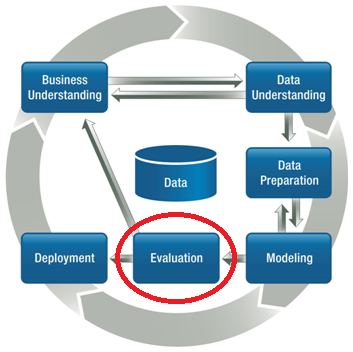
\includegraphics[width=0.5\textwidth]{./images/CRISPDM_5.png}
	\caption{CRISP-DM - Evaluation}
	\label{CRISPDM_5}
\end{figure}

In questa fase si andranno a valutare i risultati ottenuti dall'intero processo CRISP-DM fatto finora. Se tale valutazione risulta essere non positiva rispetto a ciò che il sistema si prefiggeva di fare, si passerà alla definizione di altri parametri o alla scelta di altri tipi di algoritmi per effettuare la classificazione.

\section{Valutazione rispetto agli obiettivi di business}
I risultati ottenuti, mostrati nella tabella \ref{tab:FTExtendFiltered}, possono essere considerati positivi rispetto agli obiettivi di business, in quanto supera il 99 \% di correttezza richiesto dal task \ref{task}. 

Tuttavia, al fine di tentare di migliorare ulteriormente il sistema di classificazione, sono state testate le varianti che il modello FT offriva (\emph{Alberi funzionali ai soli nodi intermedi} \ref{Alberi funzionali ai soli nodi intermedi} e \emph{Alberi funzionali ai soli nodi foglia} \ref{Alberi funzionali ai soli nodi foglia}). Per fare ciò, è stato necessario variare il parametro modelType rispettivamente in \emph{FT Inner} e \emph{FT Leaves}.

Inoltre, per completezza, è stato fatto un esperimento controllato avente n fattori con m livelli, in particolare 3 fattori:
%sono state sperimentate altre configurazioni sul dataset combinando tutti gli algoritmi definiti finora :

\textbf{Sampling} con 2 livelli:
\begin{itemize}
	\item Con SMOTE;
	\item Senza SMOTE;
\end{itemize}

\textbf{Feature Selection} con 2 livelli:
\begin{itemize}
	\item Con CfsSubsetEval;
	\item Senza CfsSubsetEval;
\end{itemize}

\textbf{Classifiers} con 3 livelli:
\begin{itemize}
	\item FT;
	\item FT-Leaves;
	\item FT-Inner.
\end{itemize}


			\begin{equation*}
			\qquad \textbf{Sampling}
			\begin{cases} 
				Con SMOTE \\~\\ Senza SMOTE 
			\end{cases}
			\end{equation*}
			\begin{equation*}
			\qquad \textbf{Feature Selection}
			\begin{cases} 
				Con CfSubsetEval \\~\\ Senza CfSubsetEval
			\end{cases}
			\end{equation*}
			\begin{equation*}
			\qquad \textbf{Classifiers}
			\begin{cases} 
			FT \\~\\ FT-Leaves \\~\\ FT-Inner
			\end{cases}
			\end{equation*}

\subsection{Risultati configurazioni}
Di seguito verranno riportati i risultati ottenuti da queste configurazioni: 


\begin{table}[htbp]
	\centering
	\resizebox{1\textwidth}{!}{%
		% Table generated by Excel2LaTeX from sheet 'FT Leaves'
			\begin{tabular}{rrrrrrrrr}
				\multicolumn{4}{c}{=== Stratified cross-validation ===} &       &       &       &       &  \\
				\multicolumn{3}{c}{=== Summary ===} &       &       &       &       &       &  \\
				&       &       &       &       &       &       &       &  \\
				Correctly Classified Instances    & 11009 & \textit{\textbf{99,0731\%}} &       & \multicolumn{4}{c}{=== Confusion Matrix ===} & \multicolumn{1}{c}{} \\
				Incorrectly Classified Instances & 103   & 0,9269\% &       &       &       &       &       &  \\
				Kappa statistic   & 0,9812 &       &       & \multicolumn{1}{c}{\textit{\textbf{Yes}}} & \multicolumn{1}{c}{\textit{\textbf{No}}} & \multicolumn{1}{c}{<--} & \multicolumn{2}{c}{Classified as} \\
				Mean absolute error & 0,0175 &       &       & \multicolumn{1}{c}{6149} & \multicolumn{1}{c}{75} &       &       &  \\
				Root mean squared error & 0,0911 &       &       & \multicolumn{1}{c}{28} & \multicolumn{1}{c}{4860} &       &       &  \\
				Relative absolute error & 3,55\% &       &       &       &       &       &       &  \\
				Root relative squared error & 18,3503\% &       &       &       &       &       &       &  \\
				Total Number of Instances      & 11112 &       &       &       &       &       &       &  \\
				Attributes & 53    &       &       &       &       &       &       &  \\
				\multicolumn{8}{c}{=== Detailed Accuracy By Class ===}        &  \\
				&       &       &       &       &       &       &       &  \\
				\multicolumn{1}{c}{} & \multicolumn{1}{c}{\textit{\textbf{TP Rate}}} & \multicolumn{1}{c}{\textit{\textbf{FP Rate}}} & \multicolumn{1}{c}{\textit{\textbf{Precision}}} & \multicolumn{1}{c}{\textit{\textbf{Recall}}} & \multicolumn{1}{c}{\textit{\textbf{F-Measure}}} & \multicolumn{1}{c}{\textit{\textbf{ROC Area}}} & \multicolumn{1}{c}{\textit{\textbf{Class}}} &  \\
				\multicolumn{1}{c}{} & \multicolumn{1}{c}{0,988} & \multicolumn{1}{c}{0,006} & \multicolumn{1}{c}{0,995} & \multicolumn{1}{c}{0,988} & \multicolumn{1}{c}{0,992} & \multicolumn{1}{c}{0,997} & \multicolumn{1}{c}{yes} &  \\
				\multicolumn{1}{c}{} & \multicolumn{1}{c}{0,994} & \multicolumn{1}{c}{0,012} & \multicolumn{1}{c}{0,985} & \multicolumn{1}{c}{0,994} & \multicolumn{1}{c}{0,99} & \multicolumn{1}{c}{0,997} & \multicolumn{1}{c}{no} &  \\
				\multicolumn{1}{c}{} & \multicolumn{1}{c}{} & \multicolumn{1}{c}{} & \multicolumn{1}{c}{} & \multicolumn{1}{c}{} & \multicolumn{1}{c}{} & \multicolumn{1}{c}{} & \multicolumn{1}{c}{} &  \\
				\multicolumn{1}{c}{\textit{\textbf{Weighted Avg.}}} & \multicolumn{1}{c}{0,991} & \multicolumn{1}{c}{0,009} & \multicolumn{1}{c}{0,991} & \multicolumn{1}{c}{0,991} & \multicolumn{1}{c}{0,991} & \multicolumn{1}{c}{0,997} & \multicolumn{1}{c}{} &  \\
			\end{tabular}%
	}
	\label{tab:FTLeavesExtendFiltered}%
	\caption{ SMOTE - CFSubsetEval - FT-Leaves}
\end{table}%

\begin{table}[htbp]
	\centering
	\resizebox{1\textwidth}{!}{%
		% Table generated by Excel2LaTeX from sheet 'FT Inner'
			\begin{tabular}{rrrrrrrrr}
				\multicolumn{4}{c}{=== Stratified cross-validation ===} &       &       &       &       &  \\
				\multicolumn{3}{c}{=== Summary ===} &       &       &       &       &       &  \\
				&       &       &       &       &       &       &       &  \\
				Correctly Classified Instances    & 11001 & \textit{\textbf{99,0011\%}} &       & \multicolumn{4}{c}{=== Confusion Matrix ===} & \multicolumn{1}{c}{} \\
				Incorrectly Classified Instances & 111   & 0,9989\% &       &       &       &       &       &  \\
				Kappa statistic   & 0,9797 &       &       & \multicolumn{1}{c}{\textit{\textbf{Yes}}} & \multicolumn{1}{c}{\textit{\textbf{No}}} & \multicolumn{1}{c}{<--} & \multicolumn{2}{c}{Classified as} \\
				Mean absolute error & 0,01  &       &       & \multicolumn{1}{c}{6150} & \multicolumn{1}{c}{74} &       &       &  \\
				Root mean squared error & 0,0999 &       &       & \multicolumn{1}{c}{37} & \multicolumn{1}{c}{4851} &       &       &  \\
				Relative absolute error & 2,03\% &       &       &       &       &       &       &  \\
				Root relative squared error & 20,1353\% &       &       &       &       &       &       &  \\
				Total Number of Instances      & 11112 &       &       &       &       &       &       &  \\
				Attributes & 53    &       &       &       &       &       &       &  \\
				\multicolumn{8}{c}{=== Detailed Accuracy By Class ===}        &  \\
				&       &       &       &       &       &       &       &  \\
				\multicolumn{1}{c}{} & \multicolumn{1}{c}{\textit{\textbf{TP Rate}}} & \multicolumn{1}{c}{\textit{\textbf{FP Rate}}} & \multicolumn{1}{c}{\textit{\textbf{Precision}}} & \multicolumn{1}{c}{\textit{\textbf{Recall}}} & \multicolumn{1}{c}{\textit{\textbf{F-Measure}}} & \multicolumn{1}{c}{\textit{\textbf{ROC Area}}} & \multicolumn{1}{c}{\textit{\textbf{Class}}} &  \\
				\multicolumn{1}{c}{} & \multicolumn{1}{c}{0,988} & \multicolumn{1}{c}{0,008} & \multicolumn{1}{c}{0,994} & \multicolumn{1}{c}{0,988} & \multicolumn{1}{c}{0,991} & \multicolumn{1}{c}{0,99} & \multicolumn{1}{c}{yes} &  \\
				\multicolumn{1}{c}{} & \multicolumn{1}{c}{0,992} & \multicolumn{1}{c}{0,012} & \multicolumn{1}{c}{0,985} & \multicolumn{1}{c}{0,992} & \multicolumn{1}{c}{0,989} & \multicolumn{1}{c}{0,99} & \multicolumn{1}{c}{no} &  \\
				\multicolumn{1}{c}{} & \multicolumn{1}{c}{} & \multicolumn{1}{c}{} & \multicolumn{1}{c}{} & \multicolumn{1}{c}{} & \multicolumn{1}{c}{} & \multicolumn{1}{c}{} & \multicolumn{1}{c}{} &  \\
				\multicolumn{1}{c}{\textit{\textbf{Weighted Avg.}}} & \multicolumn{1}{c}{0,99} & \multicolumn{1}{c}{0,009} & \multicolumn{1}{c}{0,99} & \multicolumn{1}{c}{0,99} & \multicolumn{1}{c}{0,99} & \multicolumn{1}{c}{0,99} & \multicolumn{1}{c}{} &  \\
			\end{tabular}%
	}
	\label{tab:FTInnerExtendFiltered}%
	\caption{ SMOTE - CFSubsetEval - FT-Inner}
\end{table}%

\begin{table}[htbp]
	\centering
	\resizebox{1\textwidth}{!}{%
		% Table generated by Excel2LaTeX from sheet 'FT'
			\begin{tabular}{rrrrrrrrr}
				\multicolumn{4}{c}{=== Stratified cross-validation ===} &       &       &       &       &  \\
				\multicolumn{3}{c}{=== Summary ===} &       &       &       &       &       &  \\
				&       &       &       &       &       &       &       &  \\
				Correctly Classified Instances    & 10992 & \textit{\textbf{98,9201\%}} &       & \multicolumn{4}{c}{=== Confusion Matrix ===} & \multicolumn{1}{c}{} \\
				Incorrectly Classified Instances & 120   & 1,0799\% &       &       &       &       &       &  \\
				Kappa statistic   & 0,9781 &       &       & \multicolumn{1}{c}{\textit{\textbf{Yes}}} & \multicolumn{1}{c}{\textit{\textbf{No}}} & \multicolumn{1}{c}{<--} & \multicolumn{2}{c}{Classified as} \\
				Mean absolute error & 0,0121 &       &       & \multicolumn{1}{c}{6164} & \multicolumn{1}{c}{60} &       &       &  \\
				Root mean squared error & 0,0972 &       &       & \multicolumn{1}{c}{60} & \multicolumn{1}{c}{4828} &       &       &  \\
				Relative absolute error & 2,46\% &       &       &       &       &       &       &  \\
				Root relative squared error & 19,5852\% &       &       &       &       &       &       &  \\
				Total Number of Instances      & 11112 &       &       &       &       &       &       &  \\
				Attributes & 834   &       &       &       &       &       &       &  \\
				\multicolumn{8}{c}{=== Detailed Accuracy By Class ===}        &  \\
				&       &       &       &       &       &       &       &  \\
				\multicolumn{1}{c}{} & \multicolumn{1}{c}{\textit{\textbf{TP Rate}}} & \multicolumn{1}{c}{\textit{\textbf{FP Rate}}} & \multicolumn{1}{c}{\textit{\textbf{Precision}}} & \multicolumn{1}{c}{\textit{\textbf{Recall}}} & \multicolumn{1}{c}{\textit{\textbf{F-Measure}}} & \multicolumn{1}{c}{\textit{\textbf{ROC Area}}} & \multicolumn{1}{c}{\textit{\textbf{Class}}} &  \\
				\multicolumn{1}{c}{} & \multicolumn{1}{c}{0,99} & \multicolumn{1}{c}{0,012} & \multicolumn{1}{c}{0,99} & \multicolumn{1}{c}{0,99} & \multicolumn{1}{c}{0,99} & \multicolumn{1}{c}{0,995} & \multicolumn{1}{c}{yes} &  \\
				\multicolumn{1}{c}{} & \multicolumn{1}{c}{0,988} & \multicolumn{1}{c}{0,01} & \multicolumn{1}{c}{0,988} & \multicolumn{1}{c}{0,988} & \multicolumn{1}{c}{0,988} & \multicolumn{1}{c}{0,995} & \multicolumn{1}{c}{no} &  \\
				\multicolumn{1}{c}{} & \multicolumn{1}{c}{} & \multicolumn{1}{c}{} & \multicolumn{1}{c}{} & \multicolumn{1}{c}{} & \multicolumn{1}{c}{} & \multicolumn{1}{c}{} & \multicolumn{1}{c}{} &  \\
				\multicolumn{1}{c}{\textit{\textbf{Weighted Avg.}}} & \multicolumn{1}{c}{0,989} & \multicolumn{1}{c}{0,011} & \multicolumn{1}{c}{0,989} & \multicolumn{1}{c}{0,989} & \multicolumn{1}{c}{0,989} & \multicolumn{1}{c}{0,995} & \multicolumn{1}{c}{} &  \\
			\end{tabular}%
	}
	\label{tab:FTExtend}%
	\caption{ SMOTE - Senza CFSubsetEval - FT}
\end{table}%

\begin{table}[htbp]
	\centering
	\resizebox{1\textwidth}{!}{%
		% Table generated by Excel2LaTeX from sheet 'FT Leaves'
			\begin{tabular}{rrrrrrrrr}
				\multicolumn{4}{c}{=== Stratified cross-validation ===} &       &       &       &       &  \\
				\multicolumn{3}{c}{=== Summary ===} &       &       &       &       &       &  \\
				&       &       &       &       &       &       &       &  \\
				Correctly Classified Instances    & 11028 & \textit{\textbf{99,2441\%}} &       & \multicolumn{4}{c}{=== Confusion Matrix ===} & \multicolumn{1}{c}{} \\
				Incorrectly Classified Instances & 84    & 0,7559\% &       &       &       &       &       &  \\
				Kappa statistic   & 0,9847 &       &       & \multicolumn{1}{c}{\textit{\textbf{Yes}}} & \multicolumn{1}{c}{\textit{\textbf{No}}} & \multicolumn{1}{c}{<--} & \multicolumn{2}{c}{Classified as} \\
				Mean absolute error & 0,0121 &       &       & \multicolumn{1}{c}{6166} & \multicolumn{1}{c}{58} &       &       &  \\
				Root mean squared error & 0,0798 &       &       & \multicolumn{1}{c}{26} & \multicolumn{1}{c}{4862} &       &       &  \\
				Relative absolute error & 2,45\% &       &       &       &       &       &       &  \\
				Root relative squared error & 16,0749\% &       &       &       &       &       &       &  \\
				Total Number of Instances      & 11112 &       &       &       &       &       &       &  \\
				Attributes & 834   &       &       &       &       &       &       &  \\
				\multicolumn{8}{c}{=== Detailed Accuracy By Class ===}        &  \\
				&       &       &       &       &       &       &       &  \\
				\multicolumn{1}{c}{} & \multicolumn{1}{c}{\textit{\textbf{TP Rate}}} & \multicolumn{1}{c}{\textit{\textbf{FP Rate}}} & \multicolumn{1}{c}{\textit{\textbf{Precision}}} & \multicolumn{1}{c}{\textit{\textbf{Recall}}} & \multicolumn{1}{c}{\textit{\textbf{F-Measure}}} & \multicolumn{1}{c}{\textit{\textbf{ROC Area}}} & \multicolumn{1}{c}{\textit{\textbf{Class}}} &  \\
				\multicolumn{1}{c}{} & \multicolumn{1}{c}{0,991} & \multicolumn{1}{c}{0,005} & \multicolumn{1}{c}{0,996} & \multicolumn{1}{c}{0,991} & \multicolumn{1}{c}{0,993} & \multicolumn{1}{c}{0,997} & \multicolumn{1}{c}{yes} &  \\
				\multicolumn{1}{c}{} & \multicolumn{1}{c}{0,995} & \multicolumn{1}{c}{0,009} & \multicolumn{1}{c}{0,988} & \multicolumn{1}{c}{0,995} & \multicolumn{1}{c}{0,991} & \multicolumn{1}{c}{0,997} & \multicolumn{1}{c}{no} &  \\
				\multicolumn{1}{c}{} & \multicolumn{1}{c}{} & \multicolumn{1}{c}{} & \multicolumn{1}{c}{} & \multicolumn{1}{c}{} & \multicolumn{1}{c}{} & \multicolumn{1}{c}{} & \multicolumn{1}{c}{} &  \\
				\multicolumn{1}{c}{\textit{\textbf{Weighted Avg.}}} & \multicolumn{1}{c}{0,992} & \multicolumn{1}{c}{0,007} & \multicolumn{1}{c}{0,992} & \multicolumn{1}{c}{0,992} & \multicolumn{1}{c}{0,992} & \multicolumn{1}{c}{0,997} & \multicolumn{1}{c}{} &  \\
			\end{tabular}%
	}
	\label{tab:FTLeavesExtend}%
	\caption{ SMOTE - Senza CFSubsetEval - FT-Leaves}
\end{table}%

\begin{table}[htbp]
	\centering
	\resizebox{1\textwidth}{!}{%
		% Table generated by Excel2LaTeX from sheet 'FT Inner'
		\begin{tabular}{rrrrrrrrr}
			\multicolumn{4}{c}{=== Stratified cross-validation ===} &       &       &       &       &  \\
			\multicolumn{3}{c}{=== Summary ===} &       &       &       &       &       &  \\
			&       &       &       &       &       &       &       &  \\
			Correctly Classified Instances    & 10985 & \textit{\textbf{98,8571\%}} &       & \multicolumn{4}{c}{=== Confusion Matrix ===} & \multicolumn{1}{c}{} \\
			Incorrectly Classified Instances & 127   & 1,1429\% &       &       &       &       &       &  \\
			Kappa statistic   & 0,9768 &       &       & \multicolumn{1}{c}{\textit{\textbf{Yes}}} & \multicolumn{1}{c}{\textit{\textbf{No}}} & \multicolumn{1}{c}{<--} & \multicolumn{2}{c}{Classified as} \\
			Mean absolute error & 0,0114 &       &       & \multicolumn{1}{c}{6165} & \multicolumn{1}{c}{59} &       &       &  \\
			Root mean squared error & 0,1069 &       &       & \multicolumn{1}{c}{68} & \multicolumn{1}{c}{4820} &       &       &  \\
			Relative absolute error & 2,32\% &       &       &       &       &       &       &  \\
			Root relative squared error & 21,5376\% &       &       &       &       &       &       &  \\
			Total Number of Instances      & 11112 &       &       &       &       &       &       &  \\
			Attributes & 834   &       &       &       &       &       &       &  \\
			\multicolumn{8}{c}{=== Detailed Accuracy By Class ===}        &  \\
			&       &       &       &       &       &       &       &  \\
			\multicolumn{1}{c}{} & \multicolumn{1}{c}{\textit{\textbf{TP Rate}}} & \multicolumn{1}{c}{\textit{\textbf{FP Rate}}} & \multicolumn{1}{c}{\textit{\textbf{Precision}}} & \multicolumn{1}{c}{\textit{\textbf{Recall}}} & \multicolumn{1}{c}{\textit{\textbf{F-Measure}}} & \multicolumn{1}{c}{\textit{\textbf{ROC Area}}} & \multicolumn{1}{c}{\textit{\textbf{Class}}} &  \\
			\multicolumn{1}{c}{} & \multicolumn{1}{c}{0,991} & \multicolumn{1}{c}{0,014} & \multicolumn{1}{c}{0,989} & \multicolumn{1}{c}{0,991} & \multicolumn{1}{c}{0,99} & \multicolumn{1}{c}{0,988} & \multicolumn{1}{c}{yes} &  \\
			\multicolumn{1}{c}{} & \multicolumn{1}{c}{0,986} & \multicolumn{1}{c}{0,009} & \multicolumn{1}{c}{0,988} & \multicolumn{1}{c}{0,986} & \multicolumn{1}{c}{0,987} & \multicolumn{1}{c}{0,988} & \multicolumn{1}{c}{no} &  \\
			\multicolumn{1}{c}{} & \multicolumn{1}{c}{} & \multicolumn{1}{c}{} & \multicolumn{1}{c}{} & \multicolumn{1}{c}{} & \multicolumn{1}{c}{} & \multicolumn{1}{c}{} & \multicolumn{1}{c}{} &  \\
			\multicolumn{1}{c}{\textit{\textbf{Weighted Avg.}}} & \multicolumn{1}{c}{0,989} & \multicolumn{1}{c}{0,012} & \multicolumn{1}{c}{0,989} & \multicolumn{1}{c}{0,989} & \multicolumn{1}{c}{0,989} & \multicolumn{1}{c}{0,988} & \multicolumn{1}{c}{} &  \\
		\end{tabular}%		
	}
	\label{tab:FTInnerExtend}%
	\caption{ SMOTE - Senza CFSubsetEval - FT-Inner}
\end{table}%

\begin{table}[htbp]
	\centering
	\resizebox{1\textwidth}{!}{%
		% Table generated by Excel2LaTeX from sheet 'FT'
		\begin{tabular}{rrrrrrrrr}
			\multicolumn{4}{c}{=== Stratified cross-validation ===} &       &       &       &       &  \\
			\multicolumn{3}{c}{=== Summary ===} &       &       &       &       &       &  \\
			&       &       &       &       &       &       &       &  \\
			Correctly Classified Instances    & 7898  & \textit{\textbf{98,7250\%}} &       & \multicolumn{4}{c}{=== Confusion Matrix ===} & \multicolumn{1}{c}{} \\
			Incorrectly Classified Instances & 102   & 1,2750\% &       &       &       &       &       &  \\
			Kappa statistic   & 0,9731 &       &       & \multicolumn{1}{c}{\textit{\textbf{Yes}}} & \multicolumn{1}{c}{\textit{\textbf{No}}} & \multicolumn{1}{c}{<--} & \multicolumn{2}{c}{Classified as} \\
			Mean absolute error & 0,0164 &       &       & \multicolumn{1}{c}{3046} & \multicolumn{1}{c}{66} &       &       &  \\
			Root mean squared error & 0,1072 &       &       & \multicolumn{1}{c}{36} & \multicolumn{1}{c}{4852} &       &       &  \\
			Relative absolute error & 3,4493\% &       &       &       &       &       &       &  \\
			Root relative squared error & 21,9960\% &       &       &       &       &       &       &  \\
			Total Number of Instances      & 8000  &       &       &       &       &       &       &  \\
			Attributes & 41    &       &       &       &       &       &       &  \\
			\multicolumn{8}{c}{=== Detailed Accuracy By Class ===}        &  \\
			&       &       &       &       &       &       &       &  \\
			\multicolumn{1}{c}{} & \multicolumn{1}{c}{\textit{\textbf{TP Rate}}} & \multicolumn{1}{c}{\textit{\textbf{FP Rate}}} & \multicolumn{1}{c}{\textit{\textbf{Precision}}} & \multicolumn{1}{c}{\textit{\textbf{Recall}}} & \multicolumn{1}{c}{\textit{\textbf{F-Measure}}} & \multicolumn{1}{c}{\textit{\textbf{ROC Area}}} & \multicolumn{1}{c}{\textit{\textbf{Class}}} &  \\
			\multicolumn{1}{c}{} & \multicolumn{1}{c}{0,979} & \multicolumn{1}{c}{0,007} & \multicolumn{1}{c}{0,988} & \multicolumn{1}{c}{0,979} & \multicolumn{1}{c}{0,984} & \multicolumn{1}{c}{0,99} & \multicolumn{1}{c}{yes} &  \\
			\multicolumn{1}{c}{} & \multicolumn{1}{c}{0,993} & \multicolumn{1}{c}{0,021} & \multicolumn{1}{c}{0,987} & \multicolumn{1}{c}{0,993} & \multicolumn{1}{c}{0,99} & \multicolumn{1}{c}{0,99} & \multicolumn{1}{c}{no} &  \\
			\multicolumn{1}{c}{} & \multicolumn{1}{c}{} & \multicolumn{1}{c}{} & \multicolumn{1}{c}{} & \multicolumn{1}{c}{} & \multicolumn{1}{c}{} & \multicolumn{1}{c}{} & \multicolumn{1}{c}{} &  \\
			\multicolumn{1}{c}{\textit{\textbf{Weighted Avg.}}} & \multicolumn{1}{c}{0,987} & \multicolumn{1}{c}{0,016} & \multicolumn{1}{c}{0,987} & \multicolumn{1}{c}{0,987} & \multicolumn{1}{c}{0,987} & \multicolumn{1}{c}{0,99} & \multicolumn{1}{c}{} &  \\
		\end{tabular}%
	}
	\label{tab:FTFiltered}%
	\caption{ Senza SMOTE - CFSubsetEval - FT}
\end{table}%

\begin{table}[htbp]
	\centering
	\resizebox{1\textwidth}{!}{%
		% Table generated by Excel2LaTeX from sheet 'FT Leaves'
		\begin{tabular}{rrrrrrrrr}
			\multicolumn{4}{c}{=== Stratified cross-validation ===} &       &       &       &       &  \\
			\multicolumn{3}{c}{=== Summary ===} &       &       &       &       &       &  \\
			&       &       &       &       &       &       &       &  \\
			Correctly Classified Instances    & 7901  & \textit{\textbf{98,7625\%}} &       & \multicolumn{4}{c}{=== Confusion Matrix ===} & \multicolumn{1}{c}{} \\
			Incorrectly Classified Instances & 99    & 1,2375\% &       &       &       &       &       &  \\
			Kappa statistic   & 0,9739 &       &       & \multicolumn{1}{c}{\textit{\textbf{Yes}}} & \multicolumn{1}{c}{\textit{\textbf{No}}} & \multicolumn{1}{c}{<--} & \multicolumn{2}{c}{Classified as} \\
			Mean absolute error & 0,0214 &       &       & \multicolumn{1}{c}{3044} & \multicolumn{1}{c}{68} &       &       &  \\
			Root mean squared error & 0,1027 &       &       & \multicolumn{1}{c}{31} & \multicolumn{1}{c}{4857} &       &       &  \\
			Relative absolute error & 4,4989\% &       &       &       &       &       &       &  \\
			Root relative squared error & 21,0674\% &       &       &       &       &       &       &  \\
			Total Number of Instances      & 8000  &       &       &       &       &       &       &  \\
			Attributes & 41    &       &       &       &       &       &       &  \\
			\multicolumn{8}{c}{=== Detailed Accuracy By Class ===}        &  \\
			&       &       &       &       &       &       &       &  \\
			\multicolumn{1}{c}{} & \multicolumn{1}{c}{\textit{\textbf{TP Rate}}} & \multicolumn{1}{c}{\textit{\textbf{FP Rate}}} & \multicolumn{1}{c}{\textit{\textbf{Precision}}} & \multicolumn{1}{c}{\textit{\textbf{Recall}}} & \multicolumn{1}{c}{\textit{\textbf{F-Measure}}} & \multicolumn{1}{c}{\textit{\textbf{ROC Area}}} & \multicolumn{1}{c}{\textit{\textbf{Class}}} &  \\
			\multicolumn{1}{c}{} & \multicolumn{1}{c}{0,978} & \multicolumn{1}{c}{0,006} & \multicolumn{1}{c}{0,99} & \multicolumn{1}{c}{0,978} & \multicolumn{1}{c}{0,984} & \multicolumn{1}{c}{0,997} & \multicolumn{1}{c}{yes} &  \\
			\multicolumn{1}{c}{} & \multicolumn{1}{c}{0,994} & \multicolumn{1}{c}{0,022} & \multicolumn{1}{c}{0,986} & \multicolumn{1}{c}{0,994} & \multicolumn{1}{c}{0,99} & \multicolumn{1}{c}{0,997} & \multicolumn{1}{c}{no} &  \\
			\multicolumn{1}{c}{} & \multicolumn{1}{c}{} & \multicolumn{1}{c}{} & \multicolumn{1}{c}{} & \multicolumn{1}{c}{} & \multicolumn{1}{c}{} & \multicolumn{1}{c}{} & \multicolumn{1}{c}{} &  \\
			\multicolumn{1}{c}{\textit{\textbf{Weighted Avg.}}} & \multicolumn{1}{c}{0,988} & \multicolumn{1}{c}{0,016} & \multicolumn{1}{c}{0,988} & \multicolumn{1}{c}{0,988} & \multicolumn{1}{c}{0,988} & \multicolumn{1}{c}{0,997} & \multicolumn{1}{c}{} &  \\
		\end{tabular}%
	}
	\label{tab:FTLeavesFiltered}%
	\caption{ Senza SMOTE - CFSubsetEval - FT-Leaves}
\end{table}%

\begin{table}[htbp]
	\centering
	\resizebox{1\textwidth}{!}{%
		% Table generated by Excel2LaTeX from sheet 'FT Inner'
		\begin{tabular}{rrrrrrrrr}
			\multicolumn{4}{c}{=== Stratified cross-validation ===} &       &       &       &       &  \\
			\multicolumn{3}{c}{=== Summary ===} &       &       &       &       &       &  \\
			&       &       &       &       &       &       &       &  \\
			Correctly Classified Instances    & 7896  & \textit{\textbf{98,7000\%}} &       & \multicolumn{4}{c}{=== Confusion Matrix ===} & \multicolumn{1}{c}{} \\
			Incorrectly Classified Instances & 104   & 1,3000\% &       &       &       &       &       &  \\
			Kappa statistic   & 0,9726 &       &       & \multicolumn{1}{c}{\textit{\textbf{Yes}}} & \multicolumn{1}{c}{\textit{\textbf{No}}} & \multicolumn{1}{c}{<--} & \multicolumn{2}{c}{Classified as} \\
			Mean absolute error & 0,013 &       &       & \multicolumn{1}{c}{3044} & \multicolumn{1}{c}{68} &       &       &  \\
			Root mean squared error & 0,114 &       &       & \multicolumn{1}{c}{36} & \multicolumn{1}{c}{4852} &       &       &  \\
			Relative absolute error & 2,7347\% &       &       &       &       &       &       &  \\
			Root relative squared error & 23,3871\% &       &       &       &       &       &       &  \\
			Total Number of Instances      & 8000  &       &       &       &       &       &       &  \\
			Attributes & 41    &       &       &       &       &       &       &  \\
			\multicolumn{8}{c}{=== Detailed Accuracy By Class ===}        &  \\
			&       &       &       &       &       &       &       &  \\
			\multicolumn{1}{c}{} & \multicolumn{1}{c}{\textit{\textbf{TP Rate}}} & \multicolumn{1}{c}{\textit{\textbf{FP Rate}}} & \multicolumn{1}{c}{\textit{\textbf{Precision}}} & \multicolumn{1}{c}{\textit{\textbf{Recall}}} & \multicolumn{1}{c}{\textit{\textbf{F-Measure}}} & \multicolumn{1}{c}{\textit{\textbf{ROC Area}}} & \multicolumn{1}{c}{\textit{\textbf{Class}}} &  \\
			\multicolumn{1}{c}{} & \multicolumn{1}{c}{0,978} & \multicolumn{1}{c}{0,007} & \multicolumn{1}{c}{0,988} & \multicolumn{1}{c}{0,978} & \multicolumn{1}{c}{0,983} & \multicolumn{1}{c}{0,985} & \multicolumn{1}{c}{yes} &  \\
			\multicolumn{1}{c}{} & \multicolumn{1}{c}{0,993} & \multicolumn{1}{c}{0,022} & \multicolumn{1}{c}{0,986} & \multicolumn{1}{c}{0,993} & \multicolumn{1}{c}{0,989} & \multicolumn{1}{c}{0,985} & \multicolumn{1}{c}{no} &  \\
			\multicolumn{1}{c}{} & \multicolumn{1}{c}{} & \multicolumn{1}{c}{} & \multicolumn{1}{c}{} & \multicolumn{1}{c}{} & \multicolumn{1}{c}{} & \multicolumn{1}{c}{} & \multicolumn{1}{c}{} &  \\
			\multicolumn{1}{c}{\textit{\textbf{Weighted Avg.}}} & \multicolumn{1}{c}{0,987} & \multicolumn{1}{c}{0,016} & \multicolumn{1}{c}{0,987} & \multicolumn{1}{c}{0,987} & \multicolumn{1}{c}{0,987} & \multicolumn{1}{c}{0,985} & \multicolumn{1}{c}{} &  \\
		\end{tabular}%
	}
	\label{tab:FTInnerFiltered}%
	\caption{ Senza SMOTE - CFSubsetEval - FT-Inner}
\end{table}%

\begin{table}[htbp]
	\centering
	\resizebox{1\textwidth}{!}{%
		% Table generated by Excel2LaTeX from sheet 'FT'
		\begin{tabular}{rrrrrrrrr}
			\multicolumn{4}{c}{=== Stratified cross-validation ===} &       &       &       &       &  \\
			\multicolumn{3}{c}{=== Summary ===} &       &       &       &       &       &  \\
			&       &       &       &       &       &       &       &  \\
			Correctly Classified Instances    & 7910  & \textit{\textbf{98,8750\%}} &       & \multicolumn{4}{c}{=== Confusion Matrix ===} & \multicolumn{1}{c}{} \\
			Incorrectly Classified Instances & 90    & 1,1250\% &       &       &       &       &       &  \\
			Kappa statistic   & 0,9763 &       &       & \multicolumn{1}{c}{\textit{\textbf{Yes}}} & \multicolumn{1}{c}{\textit{\textbf{No}}} & \multicolumn{1}{c}{<--} & \multicolumn{2}{c}{Classified as} \\
			Mean absolute error & 0,0139 &       &       & \multicolumn{1}{c}{3063} & \multicolumn{1}{c}{49} &       &       &  \\
			Root mean squared error & 0,1001 &       &       & \multicolumn{1}{c}{41} & \multicolumn{1}{c}{4847} &       &       &  \\
			Relative absolute error & 2,9227\% &       &       &       &       &       &       &  \\
			Root relative squared error & 20,5236\% &       &       &       &       &       &       &  \\
			Total Number of Instances      & 8000  &       &       &       &       &       &       &  \\
			Attributes & 834   &       &       &       &       &       &       &  \\
			\multicolumn{8}{c}{=== Detailed Accuracy By Class ===}        &  \\
			&       &       &       &       &       &       &       &  \\
			\multicolumn{1}{c}{} & \multicolumn{1}{c}{\textit{\textbf{TP Rate}}} & \multicolumn{1}{c}{\textit{\textbf{FP Rate}}} & \multicolumn{1}{c}{\textit{\textbf{Precision}}} & \multicolumn{1}{c}{\textit{\textbf{Recall}}} & \multicolumn{1}{c}{\textit{\textbf{F-Measure}}} & \multicolumn{1}{c}{\textit{\textbf{ROC Area}}} & \multicolumn{1}{c}{\textit{\textbf{Class}}} &  \\
			\multicolumn{1}{c}{} & \multicolumn{1}{c}{0,984} & \multicolumn{1}{c}{0,008} & \multicolumn{1}{c}{0,987} & \multicolumn{1}{c}{0,984} & \multicolumn{1}{c}{0,986} & \multicolumn{1}{c}{0,994} & \multicolumn{1}{c}{yes} &  \\
			\multicolumn{1}{c}{} & \multicolumn{1}{c}{0,992} & \multicolumn{1}{c}{0,016} & \multicolumn{1}{c}{0,99} & \multicolumn{1}{c}{0,992} & \multicolumn{1}{c}{0,991} & \multicolumn{1}{c}{0,994} & \multicolumn{1}{c}{no} &  \\
			\multicolumn{1}{c}{} & \multicolumn{1}{c}{} & \multicolumn{1}{c}{} & \multicolumn{1}{c}{} & \multicolumn{1}{c}{} & \multicolumn{1}{c}{} & \multicolumn{1}{c}{} & \multicolumn{1}{c}{} &  \\
			\multicolumn{1}{c}{\textit{\textbf{Weighted Avg.}}} & \multicolumn{1}{c}{0,989} & \multicolumn{1}{c}{0,013} & \multicolumn{1}{c}{0,989} & \multicolumn{1}{c}{0,989} & \multicolumn{1}{c}{0,989} & \multicolumn{1}{c}{0,994} & \multicolumn{1}{c}{} &  \\
		\end{tabular}%
	}
	\label{tab:FT}%
	\caption{ Senza SMOTE - Senza CFSubsetEval - FT}
\end{table}%

\begin{table}[htbp]
	\centering
	\resizebox{1\textwidth}{!}{%
		% Table generated by Excel2LaTeX from sheet 'FT Leaves'
		\begin{tabular}{rrrrrrrrr}
			\multicolumn{4}{c}{=== Stratified cross-validation ===} &       &       &       &       &  \\
			\multicolumn{3}{c}{=== Summary ===} &       &       &       &       &       &  \\
			&       &       &       &       &       &       &       &  \\
			Correctly Classified Instances    & 7926  & \textit{\textbf{99,0750\%}} &       & \multicolumn{4}{c}{=== Confusion Matrix ===} & \multicolumn{1}{c}{} \\
			Incorrectly Classified Instances & 74    & 0,9250\% &       &       &       &       &       &  \\
			Kappa statistic   & 0,9805 &       &       & \multicolumn{1}{c}{\textit{\textbf{Yes}}} & \multicolumn{1}{c}{\textit{\textbf{No}}} & \multicolumn{1}{c}{<--} & \multicolumn{2}{c}{Classified as} \\
			Mean absolute error & 0,0139 &       &       & \multicolumn{1}{c}{3064} & \multicolumn{1}{c}{48} &       &       &  \\
			Root mean squared error & 0,0913 &       &       & \multicolumn{1}{c}{26} & \multicolumn{1}{c}{4862} &       &       &  \\
			Relative absolute error & 2,9172\% &       &       &       &       &       &       &  \\
			Root relative squared error & 18,7372\% &       &       &       &       &       &       &  \\
			Total Number of Instances      & 8000  &       &       &       &       &       &       &  \\
			Attributes & 834   &       &       &       &       &       &       &  \\
			\multicolumn{8}{c}{=== Detailed Accuracy By Class ===}        &  \\
			&       &       &       &       &       &       &       &  \\
			\multicolumn{1}{c}{} & \multicolumn{1}{c}{\textit{\textbf{TP Rate}}} & \multicolumn{1}{c}{\textit{\textbf{FP Rate}}} & \multicolumn{1}{c}{\textit{\textbf{Precision}}} & \multicolumn{1}{c}{\textit{\textbf{Recall}}} & \multicolumn{1}{c}{\textit{\textbf{F-Measure}}} & \multicolumn{1}{c}{\textit{\textbf{ROC Area}}} & \multicolumn{1}{c}{\textit{\textbf{Class}}} &  \\
			\multicolumn{1}{c}{} & \multicolumn{1}{c}{0,985} & \multicolumn{1}{c}{0,005} & \multicolumn{1}{c}{0,992} & \multicolumn{1}{c}{0,985} & \multicolumn{1}{c}{0,988} & \multicolumn{1}{c}{0,998} & \multicolumn{1}{c}{yes} &  \\
			\multicolumn{1}{c}{} & \multicolumn{1}{c}{0,995} & \multicolumn{1}{c}{0,015} & \multicolumn{1}{c}{0,99} & \multicolumn{1}{c}{0,995} & \multicolumn{1}{c}{0,992} & \multicolumn{1}{c}{0,998} & \multicolumn{1}{c}{no} &  \\
			\multicolumn{1}{c}{} & \multicolumn{1}{c}{} & \multicolumn{1}{c}{} & \multicolumn{1}{c}{} & \multicolumn{1}{c}{} & \multicolumn{1}{c}{} & \multicolumn{1}{c}{} & \multicolumn{1}{c}{} &  \\
			\multicolumn{1}{c}{\textit{\textbf{Weighted Avg.}}} & \multicolumn{1}{c}{0,991} & \multicolumn{1}{c}{0,011} & \multicolumn{1}{c}{0,991} & \multicolumn{1}{c}{0,991} & \multicolumn{1}{c}{0,991} & \multicolumn{1}{c}{0,998} & \multicolumn{1}{c}{} &  \\
		\end{tabular}%		
	}
	\label{tab:FTLeaves}%
	\caption{ Senza SMOTE - Senza CFSubsetEval - FT-Leaves}
\end{table}%

\begin{table}[htbp]
	\centering
	\resizebox{1\textwidth}{!}{%
		% Table generated by Excel2LaTeX from sheet 'FT Inner'
		\begin{tabular}{rrrrrrrrr}
			\multicolumn{4}{c}{=== Stratified cross-validation ===} &       &       &       &       &  \\
			\multicolumn{3}{c}{=== Summary ===} &       &       &       &       &       &  \\
			&       &       &       &       &       &       &       &  \\
			Correctly Classified Instances    & 7908  & \textit{\textbf{98,8500\%}} &       & \multicolumn{4}{c}{=== Confusion Matrix ===} & \multicolumn{1}{c}{} \\
			Incorrectly Classified Instances & 92    & 1,1500\% &       &       &       &       &       &  \\
			Kappa statistic   & 0,9758 &       &       & \multicolumn{1}{c}{\textit{\textbf{Yes}}} & \multicolumn{1}{c}{\textit{\textbf{No}}} & \multicolumn{1}{c}{<--} & \multicolumn{2}{c}{Classified as} \\
			Mean absolute error & 0,0115 &       &       & \multicolumn{1}{c}{3064} & \multicolumn{1}{c}{48} &       &       &  \\
			Root mean squared error & 0,1072 &       &       & \multicolumn{1}{c}{44} & \multicolumn{1}{c}{4844} &       &       &  \\
			Relative absolute error & 2,4192\% &       &       &       &       &       &       &  \\
			Root relative squared error & 21,9965\% &       &       &       &       &       &       &  \\
			Total Number of Instances      & 8000  &       &       &       &       &       &       &  \\
			Attributes & 834   &       &       &       &       &       &       &  \\
			\multicolumn{8}{c}{=== Detailed Accuracy By Class ===}        &  \\
			&       &       &       &       &       &       &       &  \\
			\multicolumn{1}{c}{} & \multicolumn{1}{c}{\textit{\textbf{TP Rate}}} & \multicolumn{1}{c}{\textit{\textbf{FP Rate}}} & \multicolumn{1}{c}{\textit{\textbf{Precision}}} & \multicolumn{1}{c}{\textit{\textbf{Recall}}} & \multicolumn{1}{c}{\textit{\textbf{F-Measure}}} & \multicolumn{1}{c}{\textit{\textbf{ROC Area}}} & \multicolumn{1}{c}{\textit{\textbf{Class}}} &  \\
			\multicolumn{1}{c}{} & \multicolumn{1}{c}{0,985} & \multicolumn{1}{c}{0,009} & \multicolumn{1}{c}{0,986} & \multicolumn{1}{c}{0,985} & \multicolumn{1}{c}{0,985} & \multicolumn{1}{c}{0,988} & \multicolumn{1}{c}{yes} &  \\
			\multicolumn{1}{c}{} & \multicolumn{1}{c}{0,991} & \multicolumn{1}{c}{0,015} & \multicolumn{1}{c}{0,99} & \multicolumn{1}{c}{0,991} & \multicolumn{1}{c}{0,991} & \multicolumn{1}{c}{0,988} & \multicolumn{1}{c}{no} &  \\
			\multicolumn{1}{c}{} & \multicolumn{1}{c}{} & \multicolumn{1}{c}{} & \multicolumn{1}{c}{} & \multicolumn{1}{c}{} & \multicolumn{1}{c}{} & \multicolumn{1}{c}{} & \multicolumn{1}{c}{} &  \\
			\multicolumn{1}{c}{\textit{\textbf{Weighted Avg.}}} & \multicolumn{1}{c}{0,989} & \multicolumn{1}{c}{0,013} & \multicolumn{1}{c}{0,988} & \multicolumn{1}{c}{0,989} & \multicolumn{1}{c}{0,988} & \multicolumn{1}{c}{0,988} & \multicolumn{1}{c}{} &  \\
		\end{tabular}%
	}
	\label{tab:FTInner}%
	\caption{Senza SMOTE - Senza CFSubsetEval - FT-Inner}
\end{table}%

\section{Considerazioni}
Riepilogando, le migliori performance sul dataset utilizzato si ottengono applicando il ricampionamento, non eliminando le feature ed utilizzando come modello un albero decisionale avente solo costanti alle foglie.
Da questo si deduce che gli attributi eliminati nella feature selection pur contenendo molti missing value, non apportano rumori alla classificazione.
Un'altra considerazione da fare, riguarda il campionamento; 
\begin{table}[htbp]
	\begin{tabular}{ll}
		SMOTE - Senza CFSubsetEval - FT-Leaves	& 99.2441 \\
		Senza SMOTE - Senza CFSubsetEval - FT-Leaves & 99.0750 \\
		SMOTE - CFSubsetEval - FT-Leaves & 99.0731 \\
		SMOTE - CFSubsetEval - FT & 99.0101 \\
		SMOTE - CFSubsetEval - FT-Inner	& 99.0011 \\		
		SMOTE - Senza CFSubsetEval - FT & 98.9201 \\
		Senza SMOTE - Senza CFSubsetEval - FT & 98.8750 \\
		SMOTE - Senza CFSubsetEval - FT-Inner & 98.8571 \\
		Senza SMOTE - CFSubsetEval - FT-Leaves & 98.7625 \\
		Senza SMOTE - CFSubsetEval - FT & 98.7250 \\
		Senza SMOTE - CFSubsetEval - FT-Inner & 98.7 \\
		Senza SMOTE - Senza CFSubsetEval - FT-Inner & 98.5 \\
	\end{tabular}
\end{table}














	\clearpage
    \chapter{Deployment}
\begin{figure}[hbtp]
	\centering
	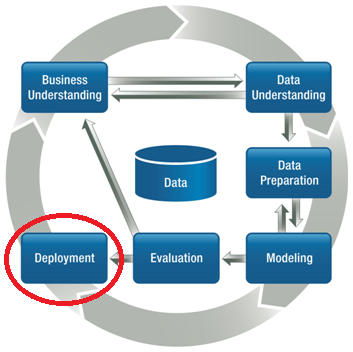
\includegraphics[width=0.9\textwidth]{./images/CRISPDM_6.png}
	\caption{CRISP-DM - Deployment}
	\label{CRISPDM_6}
\end{figure}
	\clearpage
    \chapter{Conclusioni}
	\clearpage
    \bibliographystyle{abbrvnat}
	\bibliography{mybib}

\end{document}